\documentclass{IEEEtran}
\usepackage[utf8]{vietnam}

\usepackage{cite}
\usepackage{amsmath,amssymb,amsfonts}
\usepackage{graphicx}
\usepackage{textcomp,nicefrac}
\usepackage{booktabs}
\usepackage{array}
\usepackage{tabularx}
\usepackage{url}
\usepackage{balance}

% Tinh chỉnh khoảng cách khối float để bố cục trang chặt chẽ, vừa khít không lẻ trang cuối
\setlength{\textfloatsep}{5.5pt plus 1.5pt minus 1.5pt}
\setlength{\floatsep}{4pt plus 1pt minus 1pt}
\setlength{\dbltextfloatsep}{5.5pt plus 1.5pt minus 1.5pt}
\setlength{\dblfloatsep}{4pt plus 1pt minus 1pt}
\setlength{\abovecaptionskip}{2.5pt}
\setlength{\belowcaptionskip}{-2.5pt}
\renewcommand{\topfraction}{0.90}
\renewcommand{\bottomfraction}{0.80}
\renewcommand{\textfraction}{0.08}
\renewcommand{\floatpagefraction}{0.85}
\renewcommand{\dbltopfraction}{0.90}
\renewcommand{\dblfloatpagefraction}{0.85}
\setcounter{topnumber}{3}
\setcounter{dbltopnumber}{2}
\setcounter{totalnumber}{4}

\newcolumntype{L}[1]{>{\raggedright\arraybackslash}p{#1}}
\newcolumntype{C}[1]{>{\centering\arraybackslash}p{#1}}
\newcolumntype{R}[1]{>{\raggedleft\arraybackslash}p{#1}}
\newcolumntype{Y}{>{\raggedright\arraybackslash}X}
\newcolumntype{Z}{>{\centering\arraybackslash}X}
\renewcommand{\arraystretch}{1.04}

\def\BibTeX{{\rm B\kern-.05em{\sc i\kern-.025em b}\kern-.08em
T\kern-.1667em\lower.7ex\hbox{E}\kern-.125emX}}

% Khắc phục việc gói vietnam (babel) tự dịch nhãn Abstract và rút gọn tiêu đề Tài liệu tham khảo
\AtBeginDocument{%
  \renewcommand{\abstractname}{Abstract}%
  \renewcommand{\refname}{TÀI LIỆU THAM KHẢO}%
}

\markboth{HỘI NGHỊ NGHIÊN CỨU KHOA HỌC SINH VIÊN FIT-IUH (SSRC-II'2026)}
{Nguyễn Thanh Hiệp \MakeLowercase{\textit{và cộng sự}}: UniChat: A Course-Scoped Learning Discussion Platform with a Citation-Grounded AI Assistant}

\begin{document}
\renewcommand{\abstractname}{Abstract}
\renewcommand{\refname}{TÀI LIỆU THAM KHẢO}

\title{UniChat: A Course-Scoped Learning Discussion \\ Platform with a Citation-Grounded AI Assistant}

\author{Nguyễn Thanh Hiệp$^{1}$, Hoàng Phi Hùng$^{1,*}$, Trần Thế Trung$^{1}$\\
\normalsize $^{1}$Khoa Công nghệ Thông tin, Trường Đại học Công nghiệp TP. Hồ Chí Minh, Việt Nam\\
\normalsize $^{*}$Email: 22639861.hung@student.iuh.edu.vn%
% Lưu ý: Nếu Hiệp là người đứng tên nộp bài ngày 16, đổi * sang Nguyễn Thanh Hiệp (22641211.hiep@student.iuh.edu.vn).
% Nếu nhờ Thầy nộp, đổi * sang Trần Thế Trung (tranthetrung@iuh.edu.vn).
\thanks{Bài báo được nộp tham dự Hội nghị Nghiên cứu Khoa học Sinh viên Khoa Công nghệ Thông tin lần 2 năm 2026 (SSRC-II'2026), Trường Đại học Công nghiệp TP. Hồ Chí Minh (IUH).}%
}

\maketitle

% Abstract tiếng Anh (~195 từ, chuẩn 150-200 từ, số STRICT đã chuẩn hóa, nêu thẳng 20/29 câu kiến thức nền & 24/30 chấm tay)
\begin{abstract}
In higher education, student discussions and course materials are often scattered across messaging tools lacking structured indexing and source verification, while fixed-budget Retrieval-Augmented Generation (RAG) pipelines risk context pollution, cross-course data exposure, or ungrounded answers when slides lack evidence. We present \textbf{UniChat}, a course-scoped discussion platform integrating threaded forums, reactions, and WebSocket messaging with role-based access control (RBAC) and a citation-grounded AI assistant invocable via \texttt{@UniChat}. UniChat adapts retrieval budgets across six Vietnamese query intents using dense-lexical Reciprocal Rank Fusion (RRF), an evidence gate, and post-generation citation validation. On a 120-question Vietnamese benchmark across three courses, controlled-expansion mode achieves 90.0\% decision accuracy (95\% Wilson CI: 83.3\%--94.2\%; 90.1\% on the 81-item holdout split $\mathcal{D}_{\text{holdout}}$), 86.7\% intent accuracy, 18/18 internal out-of-scope refusals (60.0\% precision, F1 0.750), and 96.1\% citation presence. On 110 valid paired queries, it outperforms normalized document-only mode (90.9\% vs.\ 73.6\%, McNemar $p = 2.1 \times 10^{-5}$); however, this gain largely stems from 29 in-scope queries absent from uploaded slides, where expansion answers 20 via background knowledge, and a 30-answer manual audit confirms 24/30 (80.0\%) directly slide-grounded. Login API load testing reaches 324.45 req/s at 200 CCU with zero errors.
\end{abstract}

\begin{IEEEkeywords}
Adaptive Retrieval, Citation Validation, Collaborative Learning Platform, Evidence Gate, Retrieval-Augmented Generation (RAG), Role-Based Access Control.
\end{IEEEkeywords}

% Tóm tắt tiếng Việt (~205 từ, khớp hoàn toàn bản tiếng Anh)
\vspace{0.15cm}
\begin{quote}
\small
\noindent\textbf{Tóm tắt}---Trong đào tạo đại học, trao đổi học thuật và học liệu thường phân tán trên các ứng dụng nhắn tin thiếu chỉ mục và đối chiếu nguồn, trong khi đường ống RAG cố định dễ gây nhiễu ngữ cảnh, lộ tài liệu giữa các lớp hoặc trả lời thiếu căn cứ khi bài giảng chưa đề cập. Bài báo trình bày \textbf{UniChat} -- nền tảng thảo luận phân nhánh, bày tỏ cảm xúc và nhắn tin WebSocket theo không gian môn học phân quyền RBAC, tích hợp trợ lý AI triệu hồi qua \texttt{@UniChat}. Hệ thống điều chỉnh ngân sách truy xuất theo 6 ý định tiếng Việt, kết hợp tìm kiếm vector--từ vựng qua RRF, cổng bằng chứng và hậu kiểm trích dẫn. Trên 120 câu hỏi tiếng Việt thuộc 3 học phần, chế độ mở rộng đạt độ chính xác quyết định 90,0\% (KTC 95\%: 83,3\%--94,2\%; tập chia độc lập $\mathcal{D}_{\text{holdout}}$ 81 câu đạt 90,1\%), nhận diện ý định 86,7\%, từ chối đúng 18/18 câu ngoài phạm vi nội bộ (chuẩn xác 60,0\%, F1 0,750) và hiện diện trích dẫn 96,1\%. Trên 110 câu ghép cặp hợp lệ, chế độ mở rộng cao hơn chế độ chỉ tài liệu đã chuẩn hóa (90,9\% so với 73,6\%, McNemar $p = 2{,}1 \times 10^{-5}$); tuy nhiên, mức tăng này chủ yếu đến từ 29 câu hỏi mà slide chưa đề cập trực tiếp -- nơi chế độ mở rộng vẫn trả lời 20 câu bằng kiến thức nền, và kiểm định thủ công 30 câu trả lời xác nhận 24/30 (80,0\%) bám trực tiếp slide. Kiểm thử tải xác thực API đăng nhập đạt 324,45 yêu cầu/giây ở 200 CCU không lỗi.

\vspace{0.12cm}
\noindent\textbf{Từ khóa}---Cổng kiểm tra bằng chứng, Kiểm soát trích dẫn, Nền tảng thảo luận học tập, Tạo văn bản tăng cường truy xuất (RAG), Truy xuất theo ý định, Xử lý ngôn ngữ tự nhiên.
\end{quote}
\vspace{0.15cm}

\section{Giới thiệu}
\label{sec:introduction}
\IEEEPARstart{T}{rong} hoạt động dạy và học ở bậc đại học, các ứng dụng giao tiếp trực tuyến (như Zalo, Facebook Groups, Discord hoặc Microsoft Teams) được sinh viên và giảng viên sử dụng phổ biến để trao đổi bài tập, thảo luận đồ án và chia sẻ học liệu. Tuy nhiên, các công cụ này được thiết kế chủ yếu cho hội thoại tức thời (ephemeral communication) nên hạn chế về khả năng tổ chức tri thức theo cấu trúc môn học. Các câu hỏi chuyên môn, giáo trình PDF, bài giảng slide và lời giải thích của giảng viên dễ bị trôi theo thời gian, khiến sinh viên gặp khó khăn khi tra cứu lại nội dung cũ và giảng viên phải giải đáp lặp lại các thắc mắc tương tự giữa các khóa học.

Sự phát triển của các Mô hình Ngôn ngữ Lớn (Large Language Models -- LLMs) kết hợp cùng kỹ thuật Tạo văn bản tăng cường truy xuất (Retrieval-Augmented Generation -- RAG) \cite{lewis2020rag, gao2023rag} mở ra hướng giải quyết khả thi cho bài toán hỏi đáp trên kho tài liệu học phần. Dù vậy, khi tích hợp một đường ống RAG cơ sở (Naive RAG) vào môi trường thảo luận học tập đa môn học, hệ thống phải đối mặt với bốn hạn chế kỹ thuật:
\begin{enumerate}
    \item \textbf{Sinh câu trả lời thiếu căn cứ khi thiếu tài liệu:} Khi người học đặt câu hỏi nằm ngoài phạm vi học liệu hiện có (out-of-scope) hoặc tài liệu chưa đề cập chi tiết, phép tìm kiếm lân cận $k$-NN trong cơ sở dữ liệu vector vẫn trả về các đoạn trích (chunk) có khoảng cách gần nhất và đưa vào mô hình sinh. Hệ quả là LLM có xu hướng suy diễn thông tin không có trong giáo trình \cite{huang2025survey}.
    \item \textbf{Ngân sách truy xuất cố định:} Nhiều hệ thống RAG cơ sở sử dụng chung một số lượng đoạn trích thu hồi cố định cho mọi loại câu hỏi. Cấu hình tĩnh này dễ gây nhiễu ngữ cảnh (context pollution) và tốn chi phí token đối với các câu hỏi định nghĩa ngắn, nhưng lại thiếu độ phủ thông tin đối với các câu hỏi so sánh nhiều khía cạnh hoặc tóm tắt chương mục \cite{jeong2024adaptiverag}.
    \item \textbf{Sự tách biệt giữa thảo luận nhóm và tra cứu tài liệu:} Sinh viên thường phải chuyển đổi qua lại giữa kênh trò chuyện nhóm và một giao diện hỏi đáp AI riêng biệt, làm gián đoạn mạch thảo luận và mất ngữ cảnh của chủ đề đang trao đổi.
    \item \textbf{Rủi ro lộ dữ liệu giữa các không gian môn học:} Trong trường đại học có nhiều lớp học và nhóm đồ án cùng chia sẻ một cơ sở dữ liệu vector, nếu truy vấn truy xuất không được ràng buộc chặt chẽ bởi danh sách tài liệu được cấp quyền từ tầng nghiệp vụ, người dùng ở nhóm này có thể gián tiếp truy xuất nội dung tài liệu riêng tư của nhóm khác.
\end{enumerate}

Nhằm góp phần giải quyết các vấn đề trên, bài báo này trình bày quá trình thiết kế, hiện thực và đánh giá thực nghiệm \textbf{UniChat} -- nền tảng thảo luận học tập tích hợp trợ lý AI trả lời có trích dẫn từ tài liệu môn học. Công trình có ba đóng góp chính:
\begin{itemize}
    \item \textbf{Kiến trúc nền tảng thảo luận gắn với không gian môn học và cơ chế \texttt{@UniChat}:} Xây dựng hệ thống tích hợp diễn đàn thảo luận phân nhánh, bày tỏ cảm xúc, nhắn tin thời gian thực qua WebSocket và quản lý học liệu theo từng không gian làm việc môn học (workspace) có kiểm soát phân quyền theo vai trò (RBAC). Trợ lý AI có thể được triệu hồi trực tiếp trong bình luận qua cú pháp \texttt{@UniChat} và chỉ truy xuất trên tập tài liệu hợp lệ $D_{\text{allowed}}$.
    \item \textbf{Áp dụng và điều chỉnh cơ chế truy xuất theo ý định kết hợp cổng kiểm tra bằng chứng:} Thiết kế bộ phân loại 6 nhóm ý định truy vấn tiếng Việt dựa trên mẫu cú pháp (độ trễ dưới $15\text{~ms}$) để điều chỉnh 5 tham số truy xuất, kết hợp tìm kiếm vector với tìm kiếm từ vựng qua thuật toán hợp nhất thứ hạng nghịch đảo (RRF), cổng kiểm tra bằng chứng (Evidence Gate) và bộ hậu kiểm trích dẫn (Citation Validator) nhằm từ chối trả lời khi tài liệu không đủ căn cứ.
    \item \textbf{Đánh giá định lượng trên bộ 120 câu hỏi tiếng Việt, phân tích loại trừ ngoại tuyến và kiểm thử tải xác thực:} Thực hiện đo kiểm tự động đầu-cuối (end-to-end) đối sánh hai chế độ vận hành trên 120 câu hỏi thuộc 3 học phần đại học, công bố công thức chỉ số, khoảng tin cậy Wilson 95\%, kiểm định ghép cặp McNemar trên 110 câu hợp lệ, phân tích loại trừ ngoại tuyến bộ điều phối ý định, kiểm định độ bám nguồn thủ công trên mẫu phân tầng 30 câu trả lời, ma trận nhầm lẫn $6 \times 6$, rà soát độ lệch nhãn--kho tài liệu và kiểm thử tải xác thực cùng WebSocket.
\end{itemize}

Phần còn lại của bài báo được tổ chức như sau: Mục~\ref{sec:related_work} tổng quan các công trình liên quan và đối sánh với UniChat; Mục~\ref{sec:system_architecture} trình bày kiến trúc phân tầng 4 lớp, công nghệ sử dụng và cơ chế phân quyền RBAC; Mục~\ref{sec:adaptive_methodology} mô tả chi tiết phương pháp phân loại ý định, truy xuất lai, cổng kiểm tra bằng chứng và hậu kiểm trích dẫn; Mục~\ref{sec:experiments_and_results} trình bày thiết kế thực nghiệm, định nghĩa chỉ số, kết quả đánh giá và bàn luận hạn chế; Mục~\ref{sec:conclusion} tóm lược kết luận và hướng phát triển.

\section{Công trình liên quan}
\label{sec:related_work}

\subsection{Các biến thể RAG có kiểm soát truy xuất và bằng chứng}
Kiến trúc RAG nguyên bản của Lewis và cộng sự \cite{lewis2020rag} thực hiện chuỗi bước tuyến tính cố định (nhúng câu hỏi -- truy xuất \textit{Top-K} -- ghép prompt -- sinh văn bản) mà không đánh giá liệu các đoạn thu hồi có thực sự chứa câu trả lời hay không \cite{gao2023rag, huang2025survey}. Để khắc phục hạn chế này, Asai và cộng sự đề xuất Self-RAG \cite{asai2024selfrag}, huấn luyện mô hình ngôn ngữ sinh thêm các token phản tư (\textit{reflection tokens}) để tự đánh giá mức độ liên quan của đoạn trích và mức độ có căn cứ của câu trả lời. Tuy nhiên, Self-RAG đòi hỏi phải tinh chỉnh (fine-tune) mô hình nền với chi phí huấn luyện lớn và khó áp dụng trực tiếp khi sử dụng các mô hình thương mại qua giao diện lập trình (API).

Theo hướng không cần tinh chỉnh mô hình sinh, Yan và cộng sự đề xuất Corrective RAG (CRAG) \cite{yan2024crag}, sử dụng một bộ đánh giá truy xuất gọn nhẹ để chấm điểm độ tin cậy của tài liệu thu hồi; khi điểm tin cậy thấp, CRAG kích hoạt nhánh tìm kiếm web bên ngoài để bổ sung nguồn. Cách tiếp cận này hiệu quả cho hỏi đáp miền mở, song việc tự động truy vấn nguồn web công cộng chưa phù hợp với bối cảnh tra cứu nội bộ môn học vốn yêu cầu câu trả lời phải bám sát giáo trình được giảng viên phê duyệt.

Gần gũi nhất với hướng tiếp cận điều phối truy xuất của chúng tôi là công trình Adaptive-RAG của Jeong và cộng sự \cite{jeong2024adaptiverag} tại hội nghị NAACL 2024. Adaptive-RAG huấn luyện một mô hình phân loại ngôn ngữ nhỏ để dự đoán độ phức tạp của câu hỏi (đơn giản, một bước hay đa bước), từ đó chọn giữa việc không truy xuất, truy xuất một lần hoặc truy xuất lặp nhiều bước. Kế thừa ý tưởng điều chỉnh chiến lược theo đặc trưng câu hỏi của Adaptive-RAG \cite{jeong2024adaptiverag}, UniChat áp dụng và điều chỉnh cho bài toán học liệu tiếng Việt theo ba điểm khác biệt kỹ thuật: (1) phân loại theo \textit{bảng phân loại 6 nhóm ý định học thuật} (định nghĩa, sự kiện, so sánh, tóm tắt, suy luận, ngoài phạm vi) thay vì chỉ phân tầng theo độ phức tạp; (2) sử dụng bộ đối sánh mẫu cú pháp tiếng Việt tất định có thời gian thực thi dưới $15\text{~ms}$ thay vì gọi thêm một mô hình phân loại học sâu; và (3) điều chỉnh đồng thời 5 tham số ngân sách truy xuất kèm cổng kiểm tra bằng chứng và bộ hậu kiểm trích dẫn trước khi lưu phản hồi.

\subsection{Nền tảng thảo luận học tập và công cụ hỏi đáp tài liệu}
Trong thực tế giảng dạy đại học, nhiều hệ thống quản lý học tập và diễn đàn lớp học gần đây đã bổ sung tính năng AI hỗ trợ người học. Theo tài liệu công khai tại thời điểm tháng 11/2026, Moodle từ phiên bản 4.5 đã tích hợp hệ thống con AI (\textit{AI subsystem}) hỗ trợ tóm tắt và sinh văn bản qua nhà cung cấp cấu hình sẵn \cite{moodle_ai}, trong khi diễn đàn lớp học Piazza đã bổ sung tính năng tóm tắt luồng hỏi đáp bằng AI từ tháng 9/2026 \cite{piazza_ai}. Tuy vậy, các hệ thống quản trị học tập này (cùng Canvas) tập trung vào quản lý khóa học và diễn đàn tổng quát, chưa tích hợp cơ chế hỏi đáp RAG kiểm soát ngưỡng bằng chứng và đối chiếu từng khẳng định với số trang và mã băm đoạn trích của học liệu nội bộ ngay trong bình luận. Ở chiều ngược lại, các công cụ hỏi đáp tài liệu bằng AI như Google NotebookLM -- vốn theo tài liệu hỗ trợ tháng 11/2026 đã hỗ trợ chia sẻ notebook theo quyền người xem/người sửa và chế độ chỉ trò chuyện \cite{notebooklm_share} -- hay ChatPDF cung cấp khả năng trích dẫn nguồn rõ ràng, song không được thiết kế kèm diễn đàn thảo luận phân nhánh, bày tỏ cảm xúc học thuật và kênh nhắn tin nhóm thời gian thực (Workchat) trong cùng một không gian môn học. UniChat kết nối hai nhóm hệ thống này bằng cách nhúng trợ lý RAG có kiểm soát quyền đọc tài liệu theo RBAC trực tiếp vào không gian thảo luận và nhắn tin của môn học.

\subsection{Nghiên cứu RAG cho tiếng Việt và đối sánh tổng hợp}
Đối với tiếng Việt, các nghiên cứu gần đây tập trung xây dựng hạ tầng dữ liệu và mô hình nền cho bài toán truy xuất tăng cường sinh. Cụ thể, Nguyen và cộng sự \cite{nguyen2024virag} đã phát triển và công bố các bộ dữ liệu mở cùng mô hình tiền huấn luyện cho hệ thống RAG và LLM tiếng Việt nhằm cải thiện năng lực hiểu và sinh văn bản học thuật bản ngữ. Bên cạnh đó, phương pháp hợp nhất thứ hạng nghịch đảo (Reciprocal Rank Fusion -- RRF) do Cormack, Clarke và Büttcher đề xuất \cite{cormack2009rrf} đã chứng minh tính ổn định cao khi kết hợp kết quả xếp hạng từ nhiều bộ truy xuất khác nhau mà không cần huấn luyện lại trọng số chuẩn hóa điểm. Kết hợp với mô hình nhúng đa ngữ \texttt{intfloat/multilingual-e5-base} \cite{wang2024multilinguale5}, UniChat áp dụng chuẩn hóa Unicode dựng sẵn (NFC), phân đoạn bảo toàn tiêu đề mục và hợp nhất RRF giữa tìm kiếm vector dày đặc với khớp từ vựng để xử lý tốt thuật ngữ chuyên ngành CNTT tiếng Việt. Bảng~\ref{tab:related_work_comparison} tóm tắt điểm khác biệt giữa UniChat và các hướng tiếp cận tiêu biểu.

\begin{table}[t]
\caption{Đối sánh UniChat với các hướng tiếp cận RAG và công cụ hiện có}
\label{tab:related_work_comparison}
\centering
\scriptsize
\setlength{\tabcolsep}{2.5pt}
\begin{tabularx}{\columnwidth}{|L{2.05cm}|C{1.15cm}|C{1.15cm}|C{1.25cm}|Y|}
\hline
\textbf{Tiêu chí kỹ thuật} & \textbf{Naive RAG \cite{lewis2020rag}} & \textbf{Self-RAG \cite{asai2024selfrag} / CRAG \cite{yan2024crag}} & \textbf{Adaptive-RAG \cite{jeong2024adaptiverag}} & \textbf{UniChat (Áp dụng \& điều chỉnh)} \\
\hline
Tiêu chí điều phối truy xuất & Cố định (\textit{Top-K} tĩnh) & Điểm phản tư / độ tin cậy & Độ phức tạp câu hỏi (3 mức) & 6 nhóm ý định học thuật tiếng Việt \\
\hline
Cơ chế phân loại đầu vào & Không & Mô hình tinh chỉnh / bộ chấm & Mô hình phân loại huấn luyện & Luật cú pháp tiếng Việt ($<15\text{~ms}$) \\
\hline
Kiểm soát trước/sau sinh & Không & Token phản tư / tìm kiếm web & Lặp truy xuất đa bước & Cổng bằng chứng \& hậu kiểm trích dẫn \\
\hline
Phân quyền đa không gian & Không định nghĩa & Không định nghĩa & Không định nghĩa & RBAC 3 vai trò, lọc $D_{\text{allowed}}$ \\
\hline
Tích hợp thảo luận nhóm & Không & Không & Không & Diễn đàn phân nhánh, \texttt{@UniChat}, WebSocket \\
\hline
\end{tabularx}
\end{table}

\section{Kiến trúc hệ thống UniChat}
\label{sec:system_architecture}

\subsection{Kiến trúc phân tầng và công nghệ sử dụng}
Hệ thống UniChat được tổ chức trong một kho mã nguồn thống nhất (monorepo) nhưng tách biệt thành \textbf{4 tầng kiến trúc} độc lập theo nguyên tắc phân tách trách nhiệm (Hình~\ref{fig:architecture}):
\begin{enumerate}
    \item \textbf{Tầng trình diễn và tương tác người dùng (Client Presentation Tier):} Xây dựng dưới dạng ứng dụng trang đơn (SPA) bằng thư viện React 18 \cite{react_docs}, ngôn ngữ TypeScript ở chế độ kiểm tra kiểu nghiêm ngặt, công cụ đóng gói Vite và TailwindCSS. Giao diện cung cấp bảng tin thảo luận phân nhánh, kênh nhắn tin nhóm, khung hỏi đáp trực tiếp qua luồng sự kiện máy chủ (Server-Sent Events -- SSE), bộ dựng công thức toán KaTeX và ngăn đối chiếu trích dẫn tài liệu gốc (\textit{Citation Drawer}).
    \item \textbf{Tầng nghiệp vụ trung tâm và phân quyền (Core API Tier):} Phát triển trên nền tảng Java Spring Boot 3.3 \cite{spring_boot_docs} vận hành trên máy ảo OpenJDK 21 LTS. Core API là thành phần trung tâm duy nhất xử lý nghiệp vụ và phân quyền (single source of truth) của toàn hệ thống: quản lý xác thực bằng JSON Web Token (JWT) theo chuẩn RFC 7519 \cite{jwt2015rfc} (ký số bất đối xứng RS256 với thời hạn 15 phút, kết hợp xoay vòng Refresh Token băm SHA-256), chuẩn hóa phản hồi lỗi theo RFC 9457 (cập nhật cho RFC 7807) \cite{rfc9457}, điều phối kênh WebSocket và kiểm tra quyền truy cập tài liệu trước khi gọi dịch vụ AI.
    \item \textbf{Tầng dịch vụ trí tuệ nhân tạo nội bộ (Private AI Service Tier):} Hiện thực bằng framework bất đồng bộ FastAPI trên Python 3.11+ kết hợp thư viện xác thực lược đồ Pydantic v2 \cite{fastapi_docs}. Dịch vụ này được cô lập trong mạng Docker nội bộ, không mở cổng trực tiếp ra Internet và không tự quyết định quyền truy cập; mọi yêu cầu từ Core API gửi sang đều phải đính kèm chữ ký dịch vụ (Service JWT) và danh sách định danh tài liệu được phép đọc ($D_{\text{allowed}}$).
    \item \textbf{Tầng lưu trữ, hàng đợi và mô hình ngôn ngữ (Data, Broker \& Model Tier):} Bao gồm bốn thành phần lưu trữ và tính toán đám mây thống nhất: (a) cơ sở dữ liệu quan hệ \textbf{Supabase PostgreSQL 15} gồm \textbf{46 bảng dữ liệu và 74 khóa ngoại} thiết kế theo dạng chuẩn 3NF, quản lý định danh, không gian môn học, bài viết, phiên hỏi đáp và vết truy xuất (\textit{retrieval traces}); (b) hàng đợi thông điệp \textbf{CloudAMQP (RabbitMQ 3.13)} và bộ nhớ đệm \textbf{Redis 7.2} phục vụ xử lý bất đồng bộ quy trình nạp tài liệu theo mô hình hướng sự kiện \cite{kleppmann2017designing} và đồng bộ sự kiện WebSocket (STOMP) với độ trễ truyền tin nội bộ đo được dưới $50\text{~ms}$ (Bảng~\ref{tab:functional_tests} và Bảng~\ref{tab:stress_results}); (c) cơ sở dữ liệu vector \textbf{Chroma Cloud} \cite{chroma_docs} thực hiện tìm kiếm đoạn văn dày đặc \cite{karpukhin2020dpr} trên vector nhúng 768 chiều từ mô hình đa ngữ \texttt{intfloat/multilingual-e5-base} \cite{wang2024multilinguale5} với chỉ mục đồ thị HNSW \cite{malkov2020hnsw} trong không gian khoảng cách cosine; và (d) mô hình sinh văn bản đám mây chính Google \textbf{Gemini 3.5 Flash} (\texttt{gemini-3.5-flash}) kèm nhà cung cấp dự phòng \textbf{The Hive} (\texttt{https://api-cdn.thehive.ai/api/v3}, mô hình \texttt{deepseek-ai/deepseek-v4.1-flash-1017}).
\end{enumerate}

\begin{figure*}[t]
\centering
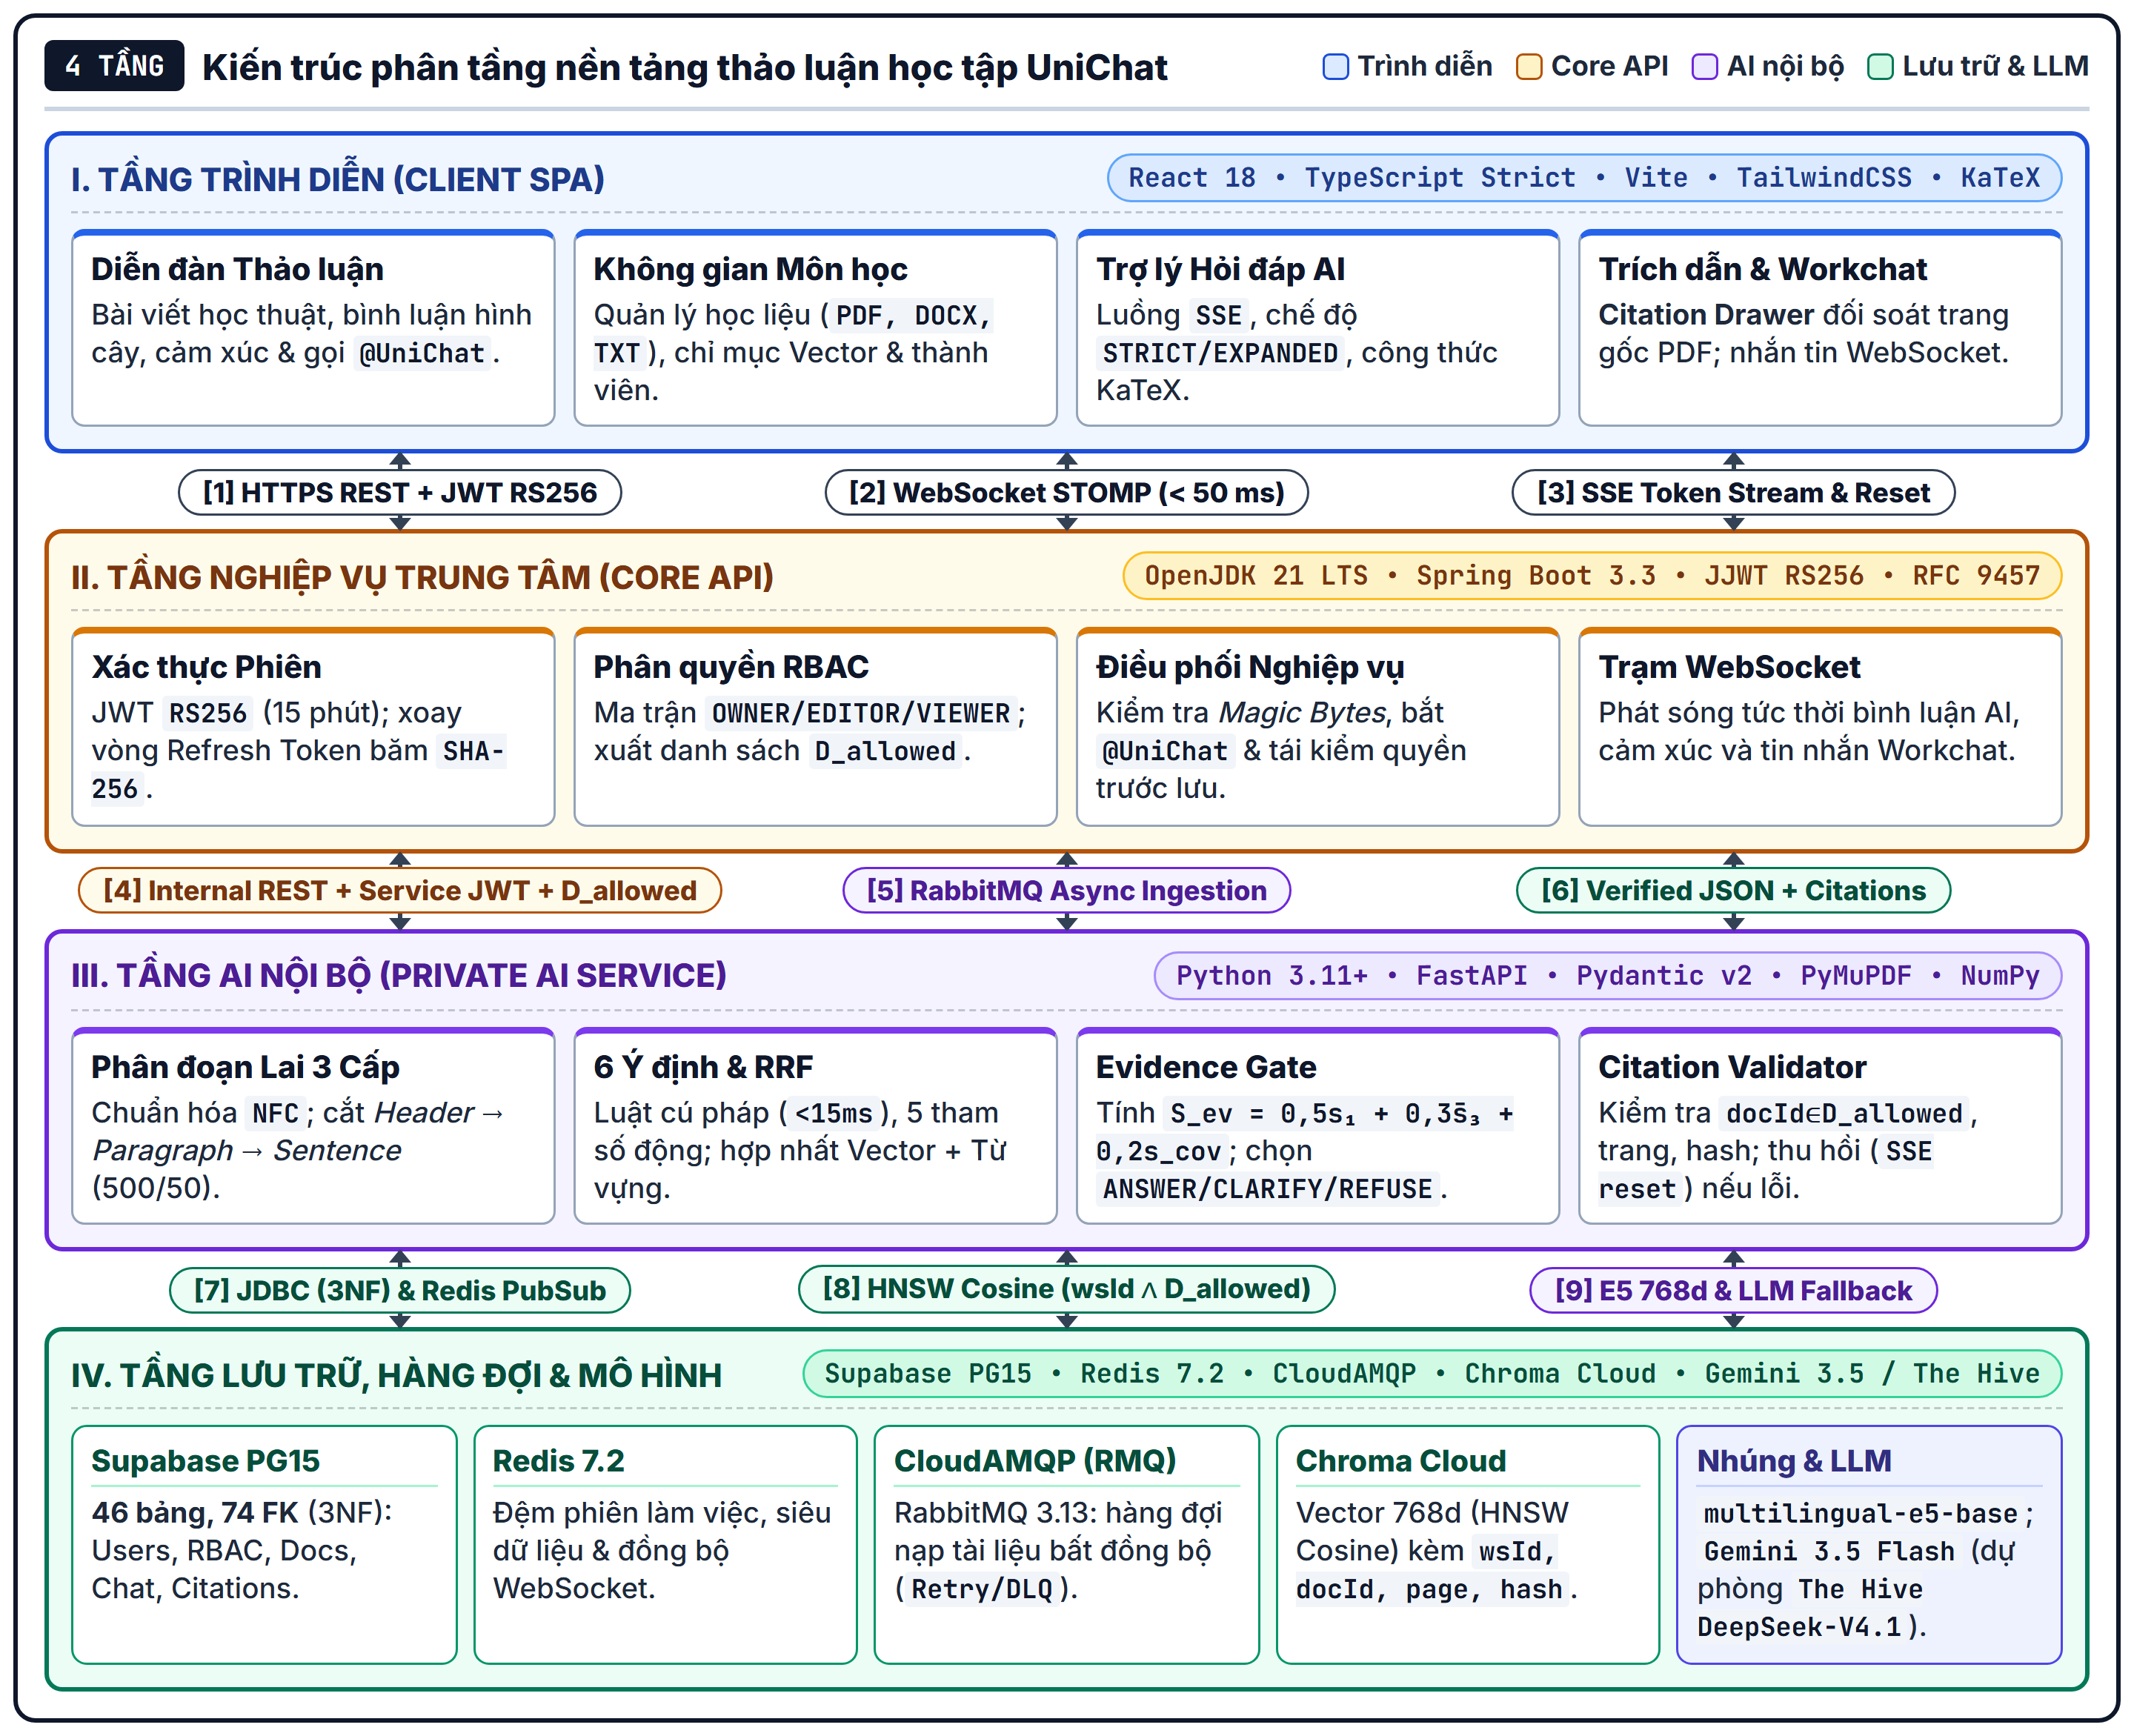
\includegraphics[width=0.92\textwidth]{architecture_overview.png}
\caption{Sơ đồ kiến trúc phân tầng 4 lớp (Tầng trình diễn SPA, Tầng nghiệp vụ trung tâm Core API trên OpenJDK 21 LTS, Tầng dịch vụ AI nội bộ và Tầng lưu trữ Supabase PostgreSQL 15 với 46 bảng / 74 khóa ngoại, CloudAMQP / RabbitMQ 3.13, Redis 7.2, Chroma Cloud, \texttt{multilingual-e5-base} và Gemini 3.5 Flash / The Hive DeepSeek-V4.1-Flash) của nền tảng UniChat.}
\label{fig:architecture}
\end{figure*}

\subsection{Ranh giới bảo mật và ma trận phân quyền (RBAC)}
Để ngăn ngừa việc truy xuất chéo tài liệu giữa các lớp học hoặc nhóm đồ án khác nhau, UniChat thiết lập ma trận phân quyền ba vai trò (\texttt{OWNER}, \texttt{EDITOR}, \texttt{VIEWER}) trong từng không gian làm việc môn học, chi tiết tại Bảng~\ref{tab:permission_matrix}.

\begin{table}[t]
\caption{Ma trận phân quyền (RBAC) trong không gian làm việc môn học UniChat}
\label{tab:permission_matrix}
\centering
\footnotesize
\setlength{\tabcolsep}{3pt}
\begin{tabularx}{\columnwidth}{|Y|C{1.15cm}|C{1.15cm}|C{1.2cm}|}
\hline
\textbf{Thao tác nghiệp vụ} & \textbf{OWNER} & \textbf{EDITOR} & \textbf{VIEWER} \\
\hline
Tạo mới hoặc xóa không gian môn học & $\checkmark$ & $\times$ & $\times$ \\
Quản lý thành viên và chỉ định vai trò & $\checkmark$ & $\times$ & $\times$ \\
Tải lên, cập nhật hoặc xóa học liệu & $\checkmark$ & $\checkmark$ & $\times$ \\
Đăng bài viết thảo luận diễn đàn & $\checkmark$ & $\checkmark$ & $\checkmark$ \\
Gửi bình luận và bày tỏ cảm xúc & $\checkmark$ & $\checkmark$ & $\checkmark$ \\
Nhắn tin trực tiếp thời gian thực (Workchat) & $\checkmark$ & $\checkmark$ & $\checkmark$ \\
Truy vấn tài liệu và gọi trợ lý AI & $\checkmark$ & $\checkmark$ & $\checkmark$ \\
Xem báo cáo đánh giá chất lượng RAG & $\checkmark$ & $\checkmark$ & $\times$ \\
\hline
\end{tabularx}
\end{table}

Mỗi khi người dùng gửi câu hỏi hoặc triệu hồi trợ lý AI trong bài thảo luận của không gian môn học $W$, Core API kiểm tra tư cách thành viên và truy vấn Supabase PostgreSQL 15 để lấy danh sách tài liệu đã xử lý hợp lệ $D_{\text{allowed}} = \{d_1, d_2, \dots, d_m\}$. Mọi truy vấn gửi tới Chroma Cloud tại AI Service đều bắt buộc áp dụng bộ lọc siêu dữ liệu:
\begin{equation}
\label{eq:rbac_filter}
\begin{aligned}
\text{Filter} =\; &(\text{wsId} == W) \land (\text{docId} \in D_{\text{allowed}}) \\
&\land (\text{status} == \text{PROCESSED})
\end{aligned}
\end{equation}
(trên sơ đồ Hình~\ref{fig:architecture} và Hình~\ref{fig:rag_pipeline}, trạng thái hoàn tất nạp \texttt{PROCESSED} được ký hiệu gọn là \texttt{OK}). Ngoài ra, mỗi ứng viên thu hồi từ Chroma Cloud còn được đối chiếu phiên bản nạp (\textit{ingestionVersion}) và mã băm SHA-256 của tệp gốc (\textit{documentContentHash}) với bản chụp siêu dữ liệu do Core API cung cấp. Cơ chế này giúp ngăn chặn các đoạn trích thuộc không gian môn học khác hoặc tài liệu đã bị thu hồi quyền lọt vào tập ngữ cảnh của mô hình sinh (kiểm chứng tại ca A-02, Bảng~\ref{tab:functional_tests}).

\subsection{Không gian thảo luận học tập và cơ chế trợ lý \texttt{@UniChat}}
Để kết nối hoạt động thảo luận nhóm với việc tra cứu học liệu, mỗi không gian môn học tích hợp ba thành phần tương tác (Hình~\ref{fig:community_ui}): (1) \textit{diễn đàn thảo luận phân nhánh} theo cấu trúc cây (\textit{nested replies}) có đính kèm tài liệu PDF/DOCX; (2) \textit{cơ chế bày tỏ cảm xúc} (\textit{Like, Insightful, Questioning}) giúp đánh dấu các câu trả lời hữu ích; và (3) \textit{kênh nhắn tin trực tiếp} (Workchat) 1-1 hoặc theo nhóm qua WebSocket.

Trong bất kỳ luồng bình luận nào, thành viên có thể gắn thẻ \texttt{@UniChat} kèm câu hỏi chuyên môn (Hình~\ref{fig:sequence_chat}). Khi đó: (1) Core API bắt sự kiện \textit{AiMentionEvent}, kiểm tra quyền thành viên và trích xuất tập $D_{\text{allowed}}$; (2) Core API đóng gói câu hỏi cùng ngữ cảnh bình luận cha gần nhất để gọi sang AI Service qua kết nối nội bộ có ký số Service JWT; (3) AI Service thực thi đường ống truy xuất theo ý định, chấm điểm cổng bằng chứng, sinh câu trả lời kèm trích dẫn và hậu kiểm; (4) Core API lưu kết quả đã kiểm chứng vào Supabase PostgreSQL 15 và phát sóng qua WebSocket tới các thành viên đang theo dõi bài viết.

\begin{figure*}[t]
\centering
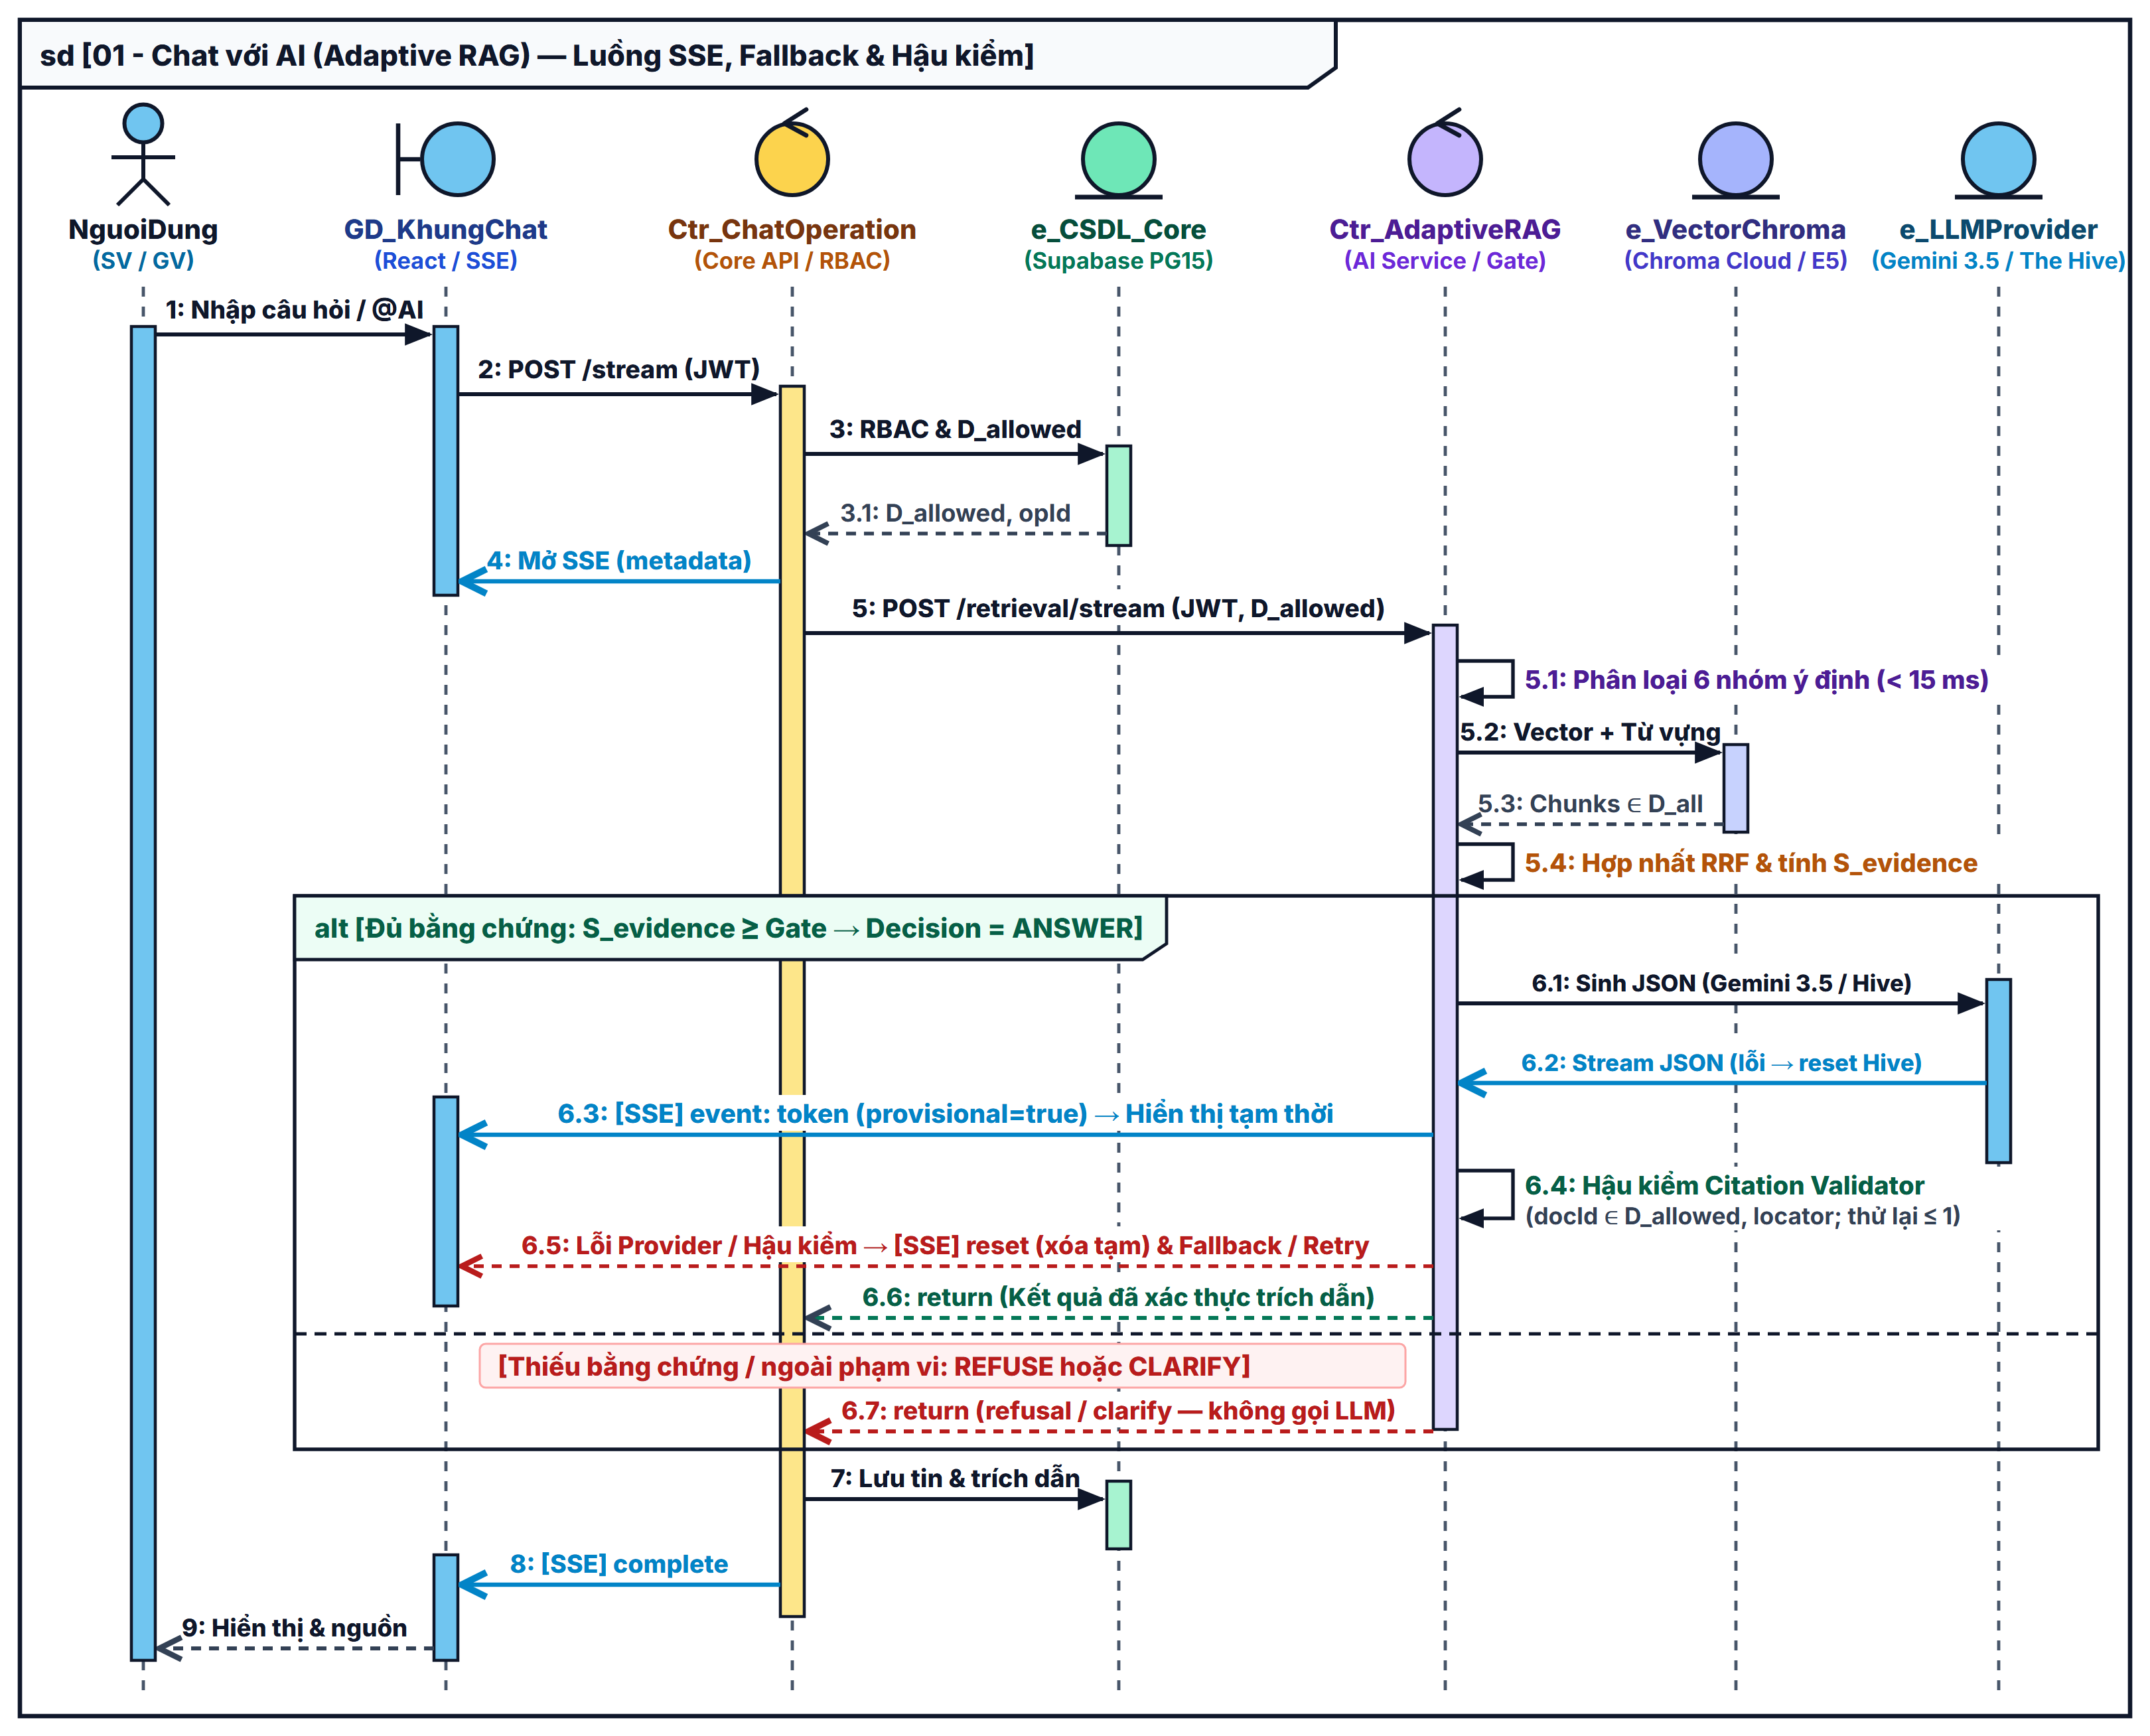
\includegraphics[width=0.92\textwidth]{sequence_chat.png}
\caption{Sơ đồ tuần tự (chuẩn UML ECB) đặc tả quy trình hỏi đáp RAG theo ý định, phát luồng token tạm thời (\texttt{provisional = true}) qua SSE, chuyển đổi dự phòng từ Gemini 3.5 Flash sang The Hive DeepSeek-V4.1-Flash (\texttt{PROVIDER\_FALLBACK}) và hậu kiểm trích dẫn (\textit{Citation Validator}) có thu hồi luồng tạm (\texttt{SSE reset}).}
\label{fig:sequence_chat}
\end{figure*}

\begin{figure*}[t]
\centering
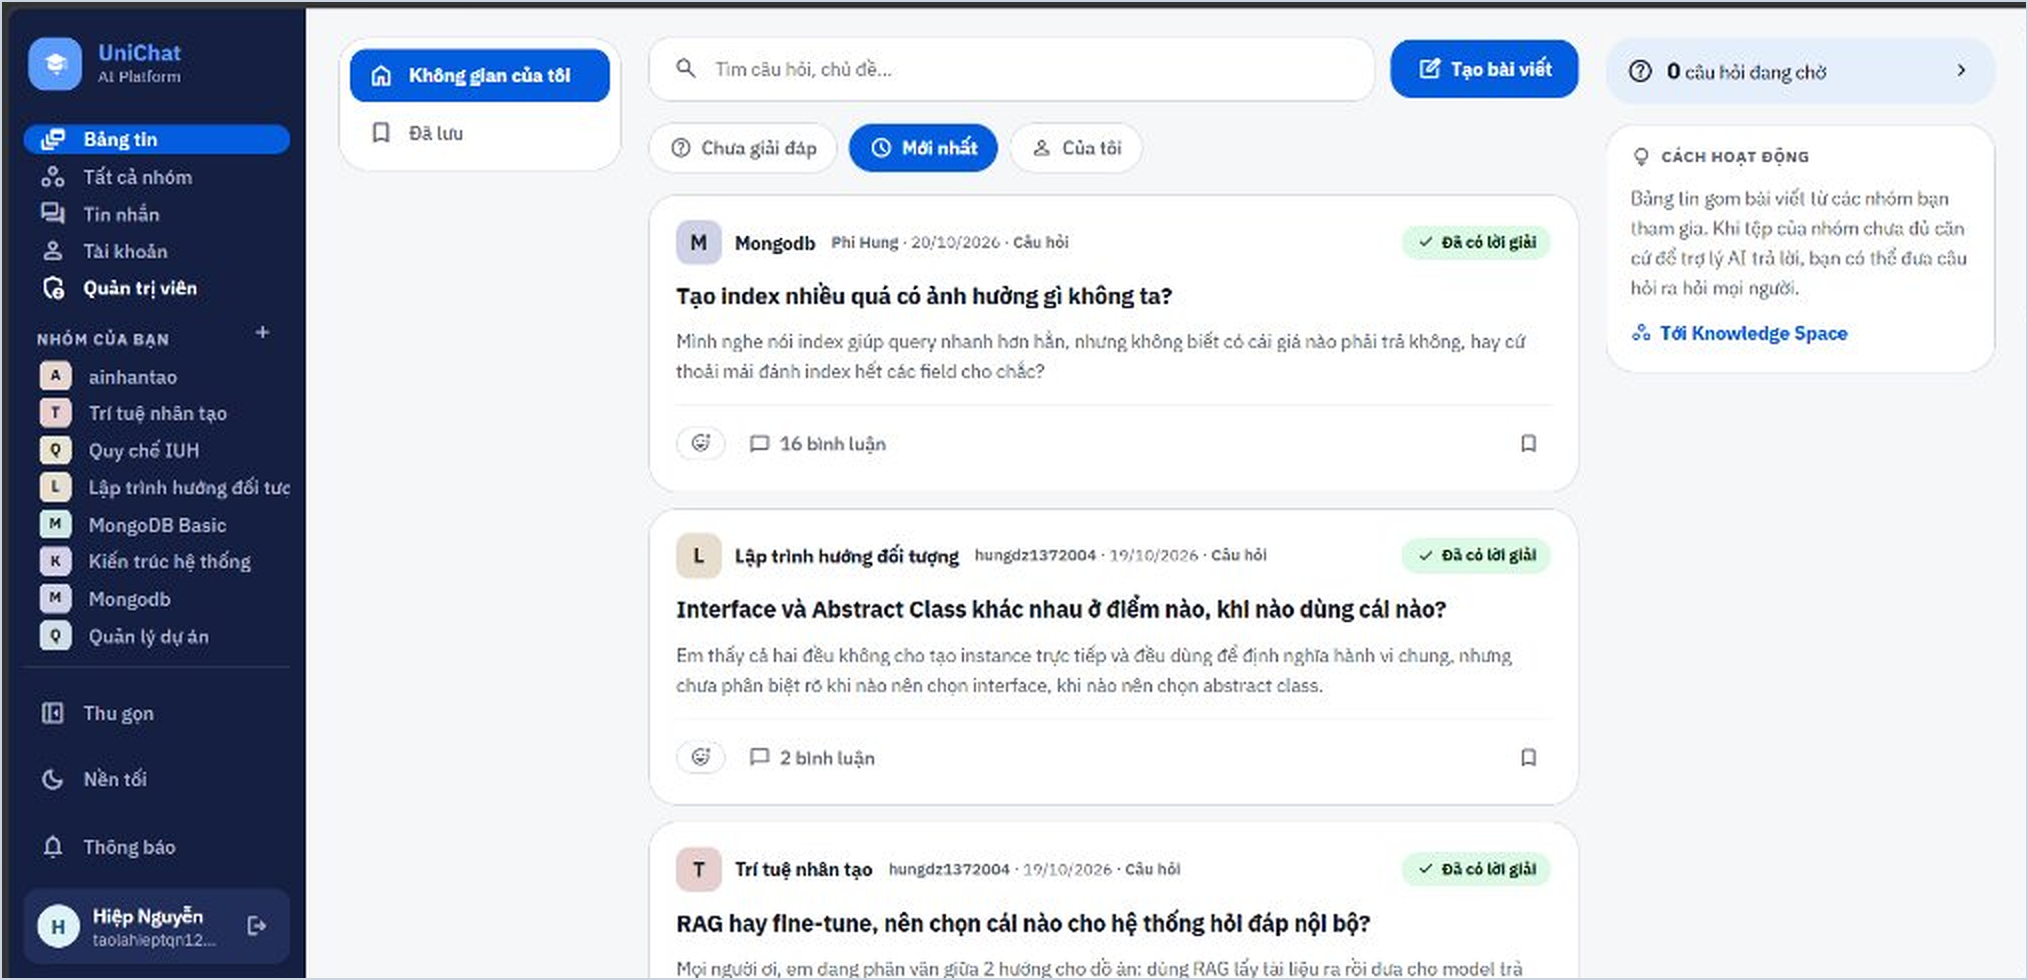
\includegraphics[width=0.92\textwidth]{community_ui.png}
\caption{Giao diện bảng tin thảo luận học tập đa không gian môn học trên UniChat: thanh điều hướng trái liệt kê các không gian môn học (\textit{Lập trình hướng đối tượng, MongoDB Basic, Quản lý dự án...}) và kênh nhắn tin; luồng trung tâm hiển thị các câu hỏi học thuật kèm trạng thái \textit{``Đã có lời giải''}, số bình luận, bày tỏ cảm xúc và bộ lọc; cột phải kết nối trực tiếp tới \textit{Knowledge Space} để chuyển tiếp giữa hỏi đáp AI và thảo luận cộng đồng.}
\label{fig:community_ui}
\end{figure*}

\section{Phương pháp truy xuất theo ý định và cổng kiểm tra bằng chứng}
\label{sec:adaptive_methodology}

\subsection{Phân loại ý định câu hỏi dựa trên mẫu cú pháp tiếng Việt}
Trước khi truy xuất, câu hỏi đầu vào (độ dài hợp lệ từ 3 đến 2.000 ký tự) được chuẩn hóa khoảng trắng và đưa về bảng mã Unicode dựng sẵn (NFC). Hệ thống tạo thêm một bản văn bản lược bỏ dấu tiếng Việt (\textit{shadow text}) chỉ dùng để đối sánh luật nhằm đảm bảo nhận diện ổn định cả khi người học gõ thiếu dấu, trong khi vẫn giữ nguyên câu hỏi gốc có dấu cho bước nhúng vector và sinh câu trả lời.

Để không phát sinh thêm một lượt gọi LLM phân loại ở đầu phễu và giữ thời gian nhận diện ý định dưới $15\text{~ms}$, chúng tôi xây dựng bộ phân loại dựa trên biểu thức chính quy nhận biết cú pháp tiếng Việt (\texttt{adaptive-retrieval-v1.yml}) kết hợp cây quyết định ưu tiên tất định qua 6 nhóm ý định:
\begin{align*}
&\text{OUT\_OF\_SCOPE} \to \text{COMPARISON} \to \text{SUMMARY} \\
&\quad \to \text{DEFINITION} \to \text{REASONING} \to \text{FACT}
\end{align*}
Ngoài ra, nếu câu hỏi thuộc dạng so sánh nhưng thiếu một trong hai vế đối sánh hoặc câu hỏi quá ngắn, chỉ chứa đại từ mơ hồ mà không có lịch sử hội thoại đi kèm, bộ phân loại sẽ chuyển thẳng sang trạng thái yêu cầu làm rõ (\texttt{CLARIFY}) trước khi truy xuất. Nhóm \texttt{FACT} đóng vai trò là nhãn mặc định (\texttt{FACT\_DEFAULT}) khi câu hỏi không khớp với 5 mẫu ưu tiên phía trước. Đặc tả của 6 nhóm ý định được trình bày tại Bảng~\ref{tab:intent_details}. Cần lưu ý rằng tầng phân loại cú pháp chỉ phát hiện các câu hỏi thuộc chủ đề ngoài phạm vi học thuật đã định nghĩa hoặc yêu cầu vượt quyền (prompt injection); còn các câu hỏi có hình thức học thuật nhưng nội dung không nằm trong học liệu của môn học sẽ được kiểm tra ở tầng truy xuất và cổng bằng chứng.

\begin{table}[t]
\caption{Đặc tả bảng phân loại 6 nhóm ý định truy vấn trong UniChat}
\label{tab:intent_details}
\centering
\scriptsize
\setlength{\tabcolsep}{3pt}
\begin{tabularx}{\columnwidth}{|L{2.25cm}|Y|Y|}
\hline
\textbf{Nhóm ý định} & \textbf{Dấu hiệu mẫu cú pháp tiếng Việt} & \textbf{Chiến lược điều phối truy xuất} \\
\hline
\texttt{OUT\_OF\_SCOPE} & Chủ đề ngoài học thuật (thời tiết, ẩm thực, tài chính, giải trí...) hoặc lệnh vượt quyền & Từ chối trả lời ngay tại tầng quy tắc, không gọi cơ sở dữ liệu vector và LLM \\
\hline
\texttt{COMPARISON} & \textit{so sánh, khác nhau, giống nhau, ưu nhược điểm, giữa A và B} & Tách khía cạnh đối sánh (facets), truy xuất song song và hợp nhất RRF \\
\hline
\texttt{SUMMARY} & \textit{tóm tắt, tổng quan, ý chính, liệt kê các, nội dung chính chương/mục} & Mở rộng ngân sách đoạn trích và số tài liệu nguồn để tăng độ bao phủ \\
\hline
\texttt{DEFINITION} & \textit{là gì, định nghĩa, khái niệm, thế nào là} & Ngân sách gọn, loại bỏ đoạn trích chỉ chứa tiêu đề mục (\textit{title-only}) \\
\hline
\texttt{REASONING} & \textit{tại sao, vì sao, nguyên nhân, ảnh hưởng, tác động, như thế nào} & Mở rộng số đoạn trích để thu thập các đoạn lập luận và giải thích \\
\hline
\texttt{FACT} & \textit{ai, khi nào, bao nhiêu, ở đâu} (hoặc nhãn mặc định \texttt{FACT\_DEFAULT}) & Truy xuất tập trung với ngưỡng tương đồng cao và ngân sách vừa phải \\
\hline
\end{tabularx}
\end{table}

\subsection{Bộ chọn tham số truy xuất theo ý định}
Ứng với mỗi nhóm ý định được xác định, bộ chọn chiến lược cấu hình 5 tham số điều khiển quá trình thu hồi và lọc bằng chứng:
\begin{itemize}
    \item \textit{Top-K}: Số lượng đoạn trích ứng viên ban đầu truy vấn từ Chroma Cloud cho mỗi biến thể truy vấn.
    \item \textit{Floor}: Ngưỡng điểm tương đồng cosine tối thiểu để chấp nhận một đoạn trích từ nhánh tìm kiếm vector.
    \item \textit{Max\_Chunks}: Số lượng đoạn trích trực tiếp tối đa được phép đóng gói vào ngữ cảnh của LLM.
    \item \textit{Min\_Sources}: Số lượng tài liệu nguồn độc lập mục tiêu cần có mặt để tính độ bao phủ nguồn.
    \item \textit{Gate}: Ngưỡng điểm bằng chứng tổng hợp tối thiểu để cho phép gọi LLM sinh câu trả lời.
\end{itemize}
Bảng~\ref{tab:strategy_params} trình bày bộ tham số chuẩn của từng nhóm ý định theo đặc tả thiết kế hệ thống. Trong trường hợp một không gian môn học chỉ có $M$ tài liệu được tải lên ($M < \textit{Min\_Sources}$), ngưỡng số nguồn hiệu dụng được tự động điều chỉnh về $\textit{Min\_Sources}_{\text{eff}} = \min(\textit{Min\_Sources}, \max(1, M))$ kèm cờ cảnh báo tổng hợp từ một nguồn duy nhất (\textit{singleSourceWarning}) để tránh từ chối sai trong các học phần chỉ dùng một tệp giáo trình tổng hợp.

\begin{table}[t]
\caption{Ma trận tham số truy xuất theo từng nhóm ý định}
\label{tab:strategy_params}
\centering
\footnotesize
\setlength{\tabcolsep}{3pt}
\begin{tabularx}{\columnwidth}{|L{2.35cm}|Z|Z|Z|Z|Z|}
\hline
\textbf{Nhóm ý định} & \textbf{\textit{Top-K}} & \textbf{\textit{Floor}} & \textbf{\textit{Max}} & \textbf{\textit{Min}} & \textbf{\textit{Gate}} \\
\hline
\texttt{DEFINITION} & 4 & 0,72 & 3 & 1 & 0,74 \\
\texttt{FACT} & 5 & 0,70 & 4 & 1 & 0,72 \\
\texttt{COMPARISON} & 10 & 0,64 & 6 & 2 & 0,68 \\
\texttt{SUMMARY} & 12 & 0,60 & 8 & 3 & 0,66 \\
\texttt{REASONING} & 12 & 0,62 & 8 & 2 & 0,68 \\
\texttt{OUT\_OF\_SCOPE} & 0 & N/A & 0 & 0 & N/A \\
\hline
\end{tabularx}
\end{table}

\subsection{Truy xuất lai và cổng kiểm tra bằng chứng (Evidence Gate)}
\label{subsec:evidence_gate}
\textbf{1) Biểu diễn độ tương đồng và truy xuất lai:}
Trong UniChat, câu hỏi $\mathbf{q}$ (gắn tiền tố \texttt{"query: "}) và mỗi đoạn trích $\mathbf{c}_i$ (gắn tiền tố \texttt{"passage: "}) được mã hóa thành vector 768 chiều đã chuẩn hóa $L_2$ ($\|\mathbf{q}\|_2 = \|\mathbf{c}_i\|_2 = 1$) bằng mô hình \texttt{intfloat/multilingual-e5-base} \cite{wang2024multilinguale5}. Khi chuẩn hóa $L_2$, độ tương đồng cosine trùng với tích vô hướng $\cos(\mathbf{q}, \mathbf{c}_i) = \mathbf{q} \cdot \mathbf{c}_i \in [-1, 1]$. Chỉ mục HNSW \cite{malkov2020hnsw} của Chroma Cloud \cite{chroma_docs} trả về khoảng cách cosine $d_{\cos}(\mathbf{q}, \mathbf{c}_i) = 1 - \cos(\mathbf{q}, \mathbf{c}_i) \in [0, 2]$. Để đưa điểm tương đồng về miền không âm $[0, 1]$, tầng truy xuất (\texttt{retrieval\_engine.py}) chuyển đổi và cắt ngưỡng dưới tại 0:
\begin{equation}
\label{eq:cosine_clip}
s_i^{\text{dense}} = \max\bigl(0,\, 1 - d_{\cos}(\mathbf{q}, \mathbf{c}_i)\bigr) \in [0, 1]
\end{equation}
Chỉ những đoạn trích vector thỏa mãn $s_i^{\text{dense}} \ge \textit{Floor}$ mới được giữ lại ở nhánh vector. Song song đó, để tránh bỏ sót các thuật ngữ chuyên ngành hoặc ký hiệu mã nguồn (như \texttt{\$lookup}, \texttt{SOLID}, \texttt{finalize()}), nhánh truy xuất từ vựng (\texttt{lexical\_retrieval.py}) tách tối đa 8 từ khóa đã loại từ dừng của câu hỏi và tìm các đoạn trích chứa từ khóa với điểm chồng lấp từ vựng:
\begin{equation}
\label{eq:lexical_score}
s_i^{\text{lex}} = \frac{|\{t \in T(\mathbf{q}) : t \in T(\mathbf{c}_i)\}|}{|T(\mathbf{q})|} \in [0, 1]
\end{equation}
trong đó các ứng viên từ vựng có $s_i^{\text{lex}} \ge 0{,}30$ được chấp nhận. Danh sách ứng viên vector và danh sách ứng viên từ vựng sau đó được hợp nhất bằng thuật toán Reciprocal Rank Fusion (RRF) \cite{cormack2009rrf} với hằng số làm trơn $k_{\text{RRF}} = 60$:
\begin{equation}
\label{eq:rrf_score}
\text{RRF}(c) = \sum_{m \in \{\text{dense}, \text{lex}\}} \frac{1}{k_{\text{RRF}} + \text{rank}_m(c)}
\end{equation}
Sau bước hợp nhất RRF và lọc bỏ các đoạn chỉ chứa tiêu đề mục (\textit{title-only}, tức đoạn có $\le 2$ dòng, $\le 12$ từ và không có dấu kết câu đối với ý định \texttt{DEFINITION}), hệ thống thu được danh sách ứng viên trực tiếp $C_{\text{direct}} = (c_1, c_2, \dots, c_L)$ đã sắp xếp theo thứ hạng, với điểm tương đồng tương ứng $s_1, s_2, \dots, s_L \in [0, 1]$.

\textbf{2) Công thức điểm bằng chứng và phân tích điều kiện chặn:}
Nếu $C_{\text{direct}} = \emptyset$ hoặc số tài liệu nguồn độc lập $N_{\text{sources}} < \textit{Min\_Sources}_{\text{eff}}$, cổng bằng chứng lập tức trả về quyết định \texttt{REFUSE}. Ngược lại, điểm bằng chứng tổng hợp $S_{\text{evidence}} \in [0, 1]$ được tính trên tối đa 3 ứng viên đứng đầu danh sách hợp nhất ($K_3 = \min(3, L)$):
\begin{equation}
\label{eq:evidence_math}
S_{\text{evidence}} = w_1 \cdot s_{\text{top}} + w_2 \cdot s_{\text{mean3}} + w_3 \cdot s_{\text{cov}}
\end{equation}
với $s_{\text{top}} = s_1$, $s_{\text{mean3}} = \frac{1}{K_3}\sum_{j=1}^{K_3} s_j$, và điểm bao phủ nguồn:
\begin{equation}
\label{eq:coverage_math}
s_{\text{cov}} = \min \left( 1{,}0, \, \frac{N_{\text{sources}}}{\textit{Min\_Sources}_{\text{eff}}} \right)
\end{equation}
Bộ trọng số $\{w_1, w_2, w_3\} = \{0{,}50; 0{,}30; 0{,}20\}$ ($w_1 + w_2 + w_3 = 1{,}0$) được chọn trên tập phát triển (development set). Hệ thống quyết định \texttt{ANSWER} khi $S_{\text{evidence}} \ge \textit{Gate}$, và \texttt{REFUSE} khi $S_{\text{evidence}} < \textit{Gate}$.

Một tính chất toán học quan trọng cần được làm rõ: tại thời điểm tính công thức~(\ref{eq:evidence_math}), hệ thống đã kiểm tra điều kiện đủ số nguồn ($N_{\text{sources}} \ge \textit{Min\_Sources}_{\text{eff}}$, tức $s_{\text{cov}} = 1{,}0$). Do đó, nếu cả $K_3$ ứng viên đầu tiên đều xuất phát từ nhánh tìm kiếm vector thuần túy ($s_j \ge \textit{Floor}$ với mọi $j \in \{1, \dots, K_3\}$), thì điểm bằng chứng luôn thỏa mãn cận dưới:
\begin{equation}
\label{eq:floor_bound}
S_{\text{evidence}} \ge (w_1 + w_2)\cdot \textit{Floor} + w_3 \cdot 1{,}0 = 0{,}80\cdot \textit{Floor} + 0{,}20
\end{equation}
Với mọi nhóm ý định trong Bảng~\ref{tab:strategy_params}, giá trị $0{,}80\cdot \textit{Floor} + 0{,}20$ đều lớn hơn ngưỡng $\textit{Gate}$ (ví dụ: ở nhóm \texttt{DEFINITION}, $0{,}80 \times 0{,}72 + 0{,}20 = 0{,}776 > 0{,}74$; ở nhóm \texttt{FACT}, $0{,}80 \times 0{,}70 + 0{,}20 = 0{,}760 > 0{,}72$; ở nhóm \texttt{SUMMARY}, $0{,}80 \times 0{,}60 + 0{,}20 = 0{,}680 > 0{,}66$). Điều này có nghĩa là trong trường hợp chỉ có các đoạn trích vector thuần túy vượt ngưỡng \textit{Floor}, quyết định của tầng truy xuất thực chất đã được xác định bởi ba điều kiện: (i) có ít nhất một đoạn trích không phải tiêu đề vượt ngưỡng \textit{Floor}, (ii) đủ số nguồn tài liệu tối thiểu, và (iii) vượt qua bộ hậu kiểm trích dẫn. Ngưỡng \textit{Gate} trong công thức~(\ref{eq:evidence_math}) chỉ thực sự phát huy vai trò chặn bổ sung khi danh sách hợp nhất RRF $C_{\text{direct}}$ chứa các ứng viên từ nhánh khớp từ vựng có điểm $0{,}30 \le s_j^{\text{lex}} < \textit{Floor}$ làm kéo giảm $s_{\text{top}}$ hoặc $s_{\text{mean3}}$.

\textbf{3) Ví dụ số minh họa cơ chế tính điểm:}
Để minh họa bằng số cụ thể cho công thức~(\ref{eq:evidence_math}) và bất đẳng thức~(\ref{eq:floor_bound}), xét hai kịch bản số giả lập lấy cảm hứng từ hai câu hỏi trong không gian môn học \textit{Lập trình hướng đối tượng} (số điểm $s_i$ minh họa nguyên lý tính toán, không trích từ tệp DOM kết quả ngày 27/09/2026 vốn không lưu điểm thành phần từng đoạn trích):
\begin{itemize}
    \item \textit{Kịch bản 1 (Chấp nhận trả lời -- \texttt{ANSWER}):} Câu hỏi $q_1 =$ \textit{``Đa hình trong lập trình hướng đối tượng là gì?''}. Bộ phân loại khớp mẫu \texttt{la gi} và gán nhãn \texttt{DEFINITION} ($< 15\text{~ms}$), chọn cấu hình $(\textit{Top-K}=4, \textit{Floor}=0{,}72, \textit{Max}=3, \textit{Min}=1, \textit{Gate}=0{,}74)$. Giả sử nhánh vector thu hồi 3 đoạn trích hợp lệ từ giáo trình có điểm tương đồng $s_1 = 0{,}84, s_2 = 0{,}79, s_3 = 0{,}75$ (đều $\ge 0{,}72$ và không phải đoạn chỉ chứa tiêu đề); $N_{\text{sources}} = 1 \implies s_{\text{cov}} = 1{,}0$. Điểm bằng chứng đạt $S_{\text{evidence}} = 0{,}50 \times 0{,}84 + 0{,}30 \times \frac{0{,}84+0{,}79+0{,}75}{3} + 0{,}20 \times 1{,}0 = 0{,}420 + 0{,}238 + 0{,}200 = 0{,}858 \ge 0{,}74 \implies \text{\texttt{ANSWER}}$.
    \item \textit{Kịch bản 2 (Chặn tại cổng bằng chứng -- \texttt{REFUSE} và hạn chế ghép hai thang điểm):} Xét câu hỏi $q_2 =$ \textit{``Phương thức finalize() trong Java có tác dụng gì?''} (tương ứng mã ca \texttt{BM-OOP-FACT-004}). Bộ phân loại gán nhãn \texttt{FACT} ($\textit{Floor}=0{,}70, \textit{Gate}=0{,}72$). Cần lưu ý thẳng thắn rằng trong bộ 120 câu, mã ca này bị gán nhãn gốc \texttt{ANSWER} dù slide Java nhập môn tải lên chỉ đề cập khối \texttt{finally} trong xử lý ngoại lệ chứ không có mục giải thích \texttt{finalize()}; do đó theo nhãn gốc đây là một ca lỗi từ chối (xem phân tích lệch nhãn tại Mục~\ref{subsec:intent_and_error_analysis}). Về cơ chế tính điểm, khi nhánh vector thu hồi 1 đoạn sát ngưỡng $s_1^{\text{dense}} = 0{,}705 \ge 0{,}70$ và nhánh từ vựng đưa vào 2 đoạn khớp từ rời rạc có điểm $s_2^{\text{lex}} = 0{,}40$ và $s_3^{\text{lex}} = 0{,}33$ ($\ge 0{,}30$) trên 1 tài liệu nguồn ($s_{\text{cov}} = 1{,}0$), ta có $s_{\text{top}} = 0{,}705$ và $s_{\text{mean3}} = (0{,}705 + 0{,}400 + 0{,}330)/3 = 0{,}478$, dẫn tới $S_{\text{evidence}} = 0{,}50 \times 0{,}705 + 0{,}30 \times 0{,}478 + 0{,}20 \times 1{,}0 = 0{,}696 < 0{,}72$ (\textit{Gate}) và cổng kích hoạt \texttt{REFUSE}. Kịch bản này đồng thời bộc lộ một hạn chế kiến trúc hiện hành: hai thang điểm có bản chất phân bố khác nhau -- độ tương đồng cosine $s^{\text{dense}}$ và tỷ lệ chồng lấp từ vựng $s^{\text{lex}}$ -- đang được đưa trực tiếp vào cùng công thức tuyến tính~(\ref{eq:evidence_math}) dưới một ngưỡng \textit{Gate} duy nhất, nên ứng viên từ vựng có thể kéo thấp $s_{\text{mean3}}$ ngay cả khi đoạn đứng đầu vượt ngưỡng vector.
\end{itemize}

\begin{figure*}[t]
\centering
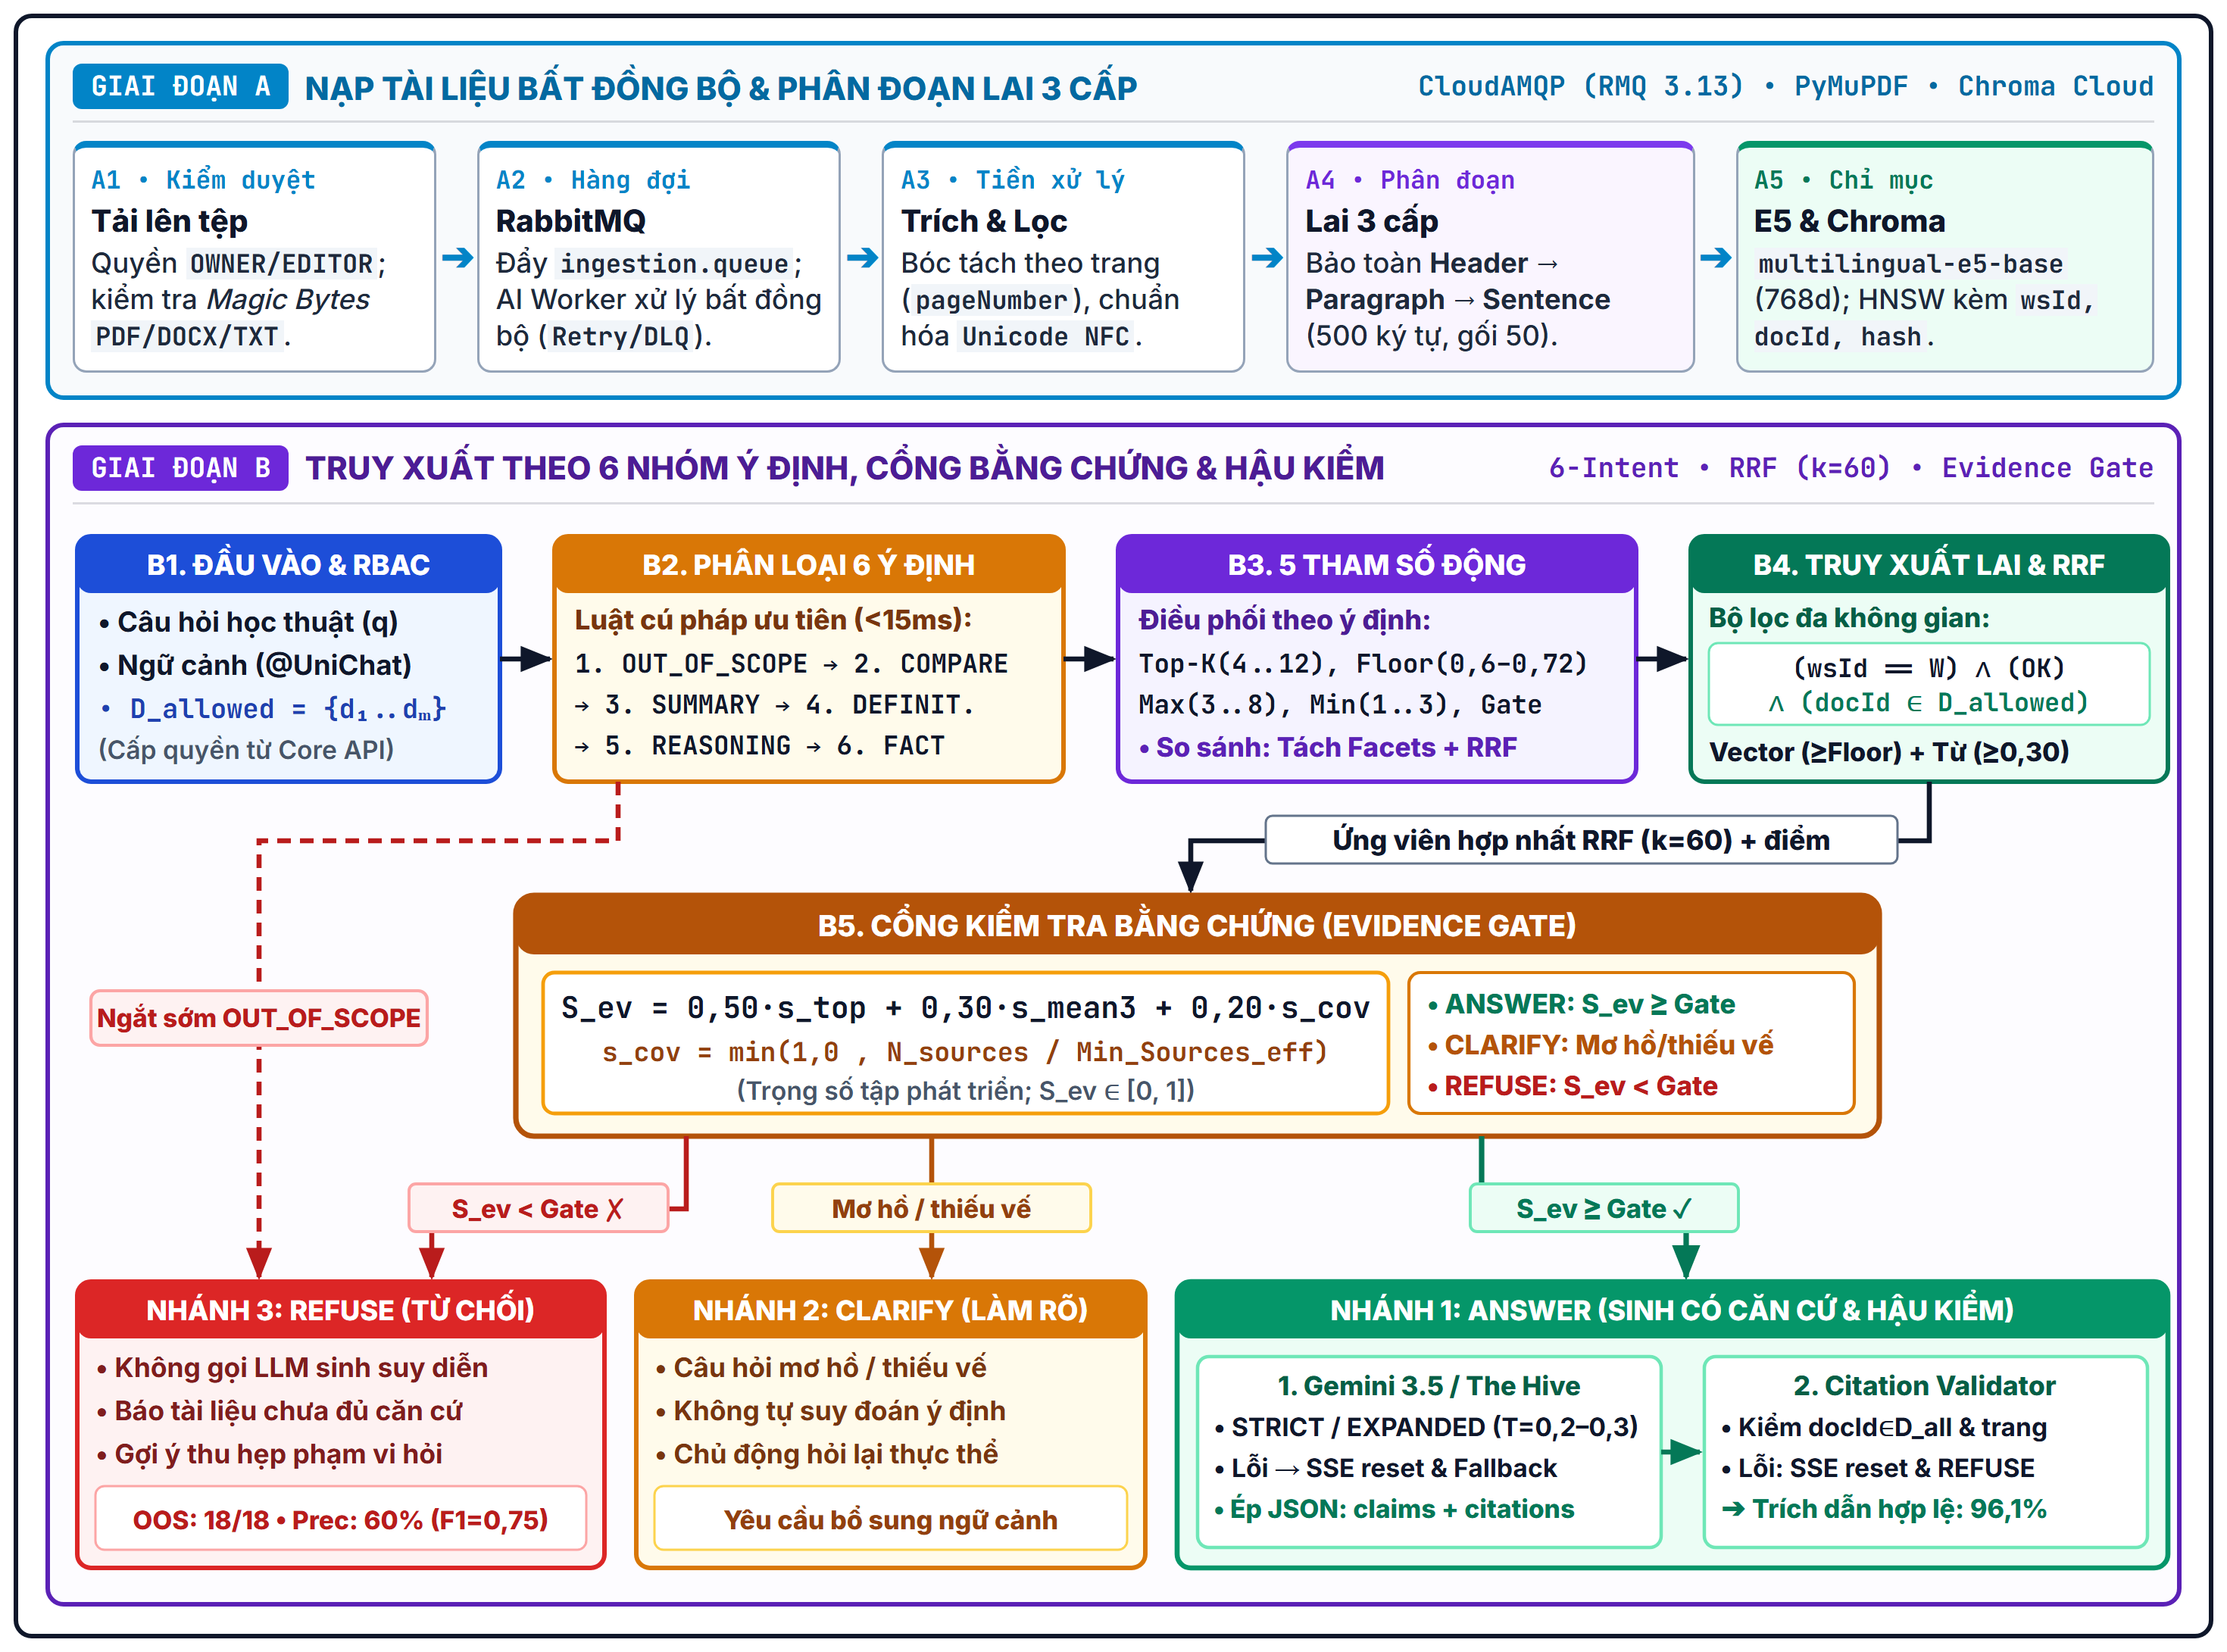
\includegraphics[width=0.92\textwidth]{rag_pipeline.png}
\caption{Quy trình nạp tài liệu bất đồng bộ phân đoạn lai 3 cấp (Giai đoạn A, sử dụng mô hình nhúng \texttt{multilingual-e5-base}) và đường ống truy xuất theo 6 nhóm ý định kết hợp hợp nhất RRF, cổng kiểm tra bằng chứng và hậu kiểm trích dẫn (Giai đoạn B).}
\label{fig:rag_pipeline}
\end{figure*}

\subsection{Phân đoạn văn bản lai 3 cấp và tách khía cạnh truy vấn}
Trong giai đoạn nạp tài liệu (Hình~\ref{fig:rag_pipeline}, Giai đoạn A), tệp PDF/DOCX/TXT sau khi kiểm tra chữ ký định dạng tệp (\textit{magic bytes}) và trích xuất văn bản theo từng trang được đưa qua bộ phân đoạn lai 3 cấp (\textit{Header $\to$ Paragraph $\to$ Sentence}, kích thước mục tiêu 500 ký tự, độ gối đầu 50 ký tự). Bộ phân đoạn nhận diện dòng tiêu đề mục để gắn vào siêu dữ liệu \texttt{section\_heading} của từng đoạn con, giúp đoạn trích giữ được ngữ cảnh đề mục khi nhúng bằng \texttt{multilingual-e5-base}.

Đối với các câu hỏi thuộc nhóm \texttt{COMPARISON}, bộ lập kế hoạch truy vấn (\texttt{question\_planner.py}) tách câu hỏi gốc thành các khía cạnh con độc lập (\textit{facets}, ví dụ khía cạnh về \textit{Scrum} và khía cạnh về \textit{Kanban}). Từng khía cạnh được truy xuất độc lập dưới cùng bộ lọc quyền $D_{\text{allowed}}$, sau đó hàm hợp nhất RRF (\texttt{evidence\_ranking.py}) giữ lại ứng viên tốt nhất của mỗi khía cạnh trước khi lấp đầy ngân sách \textit{Max\_Chunks} và bổ sung tối đa 2 đoạn trích lân cận cùng tài liệu (\textit{neighbor expansion}) để làm rõ ngữ cảnh.

\subsection{Phát luồng tạm thời, hậu kiểm trích dẫn và quản lý hội thoại}
\label{subsec:streaming_and_validation}
\textbf{1) Cơ chế đồng tồn tại giữa đầu ra JSON và luồng hiển thị SSE:}
Một yêu cầu kỹ thuật đặt ra là hệ thống vừa phải kiểm tra chặt chẽ mối liên kết giữa từng khẳng định (\textit{claim}) với mã tài liệu nguồn, vừa phải hiển thị văn bản từng phần lên giao diện để người học không phải chờ trắng màn hình trong suốt quá trình LLM suy luận. Để giải quyết vấn đề này, mô hình chính Google Gemini 3.5 Flash (\texttt{gemini-3.5-flash}) được ép sinh đầu ra theo lược đồ JSON nghiêm ngặt (\texttt{GeneratedAnswer}) gồm danh sách các phần (\texttt{sections}: \texttt{DOCUMENT} hoặc \texttt{EXTERNAL}), trong đó mỗi phần chứa các cặp $\{\texttt{text}, \texttt{citationIds}\}$.

Trong khi LLM đang truyền các mảnh chuỗi JSON về AI Service, bộ tách luồng trạng thái hữu hạn \texttt{IncrementalClaimExtractor} (\texttt{stream\_provider.py}) dò tìm khóa \texttt{"text": "} trong bộ đệm, giải mã ký tự thoát (unescape) theo thời gian thực (đồng thời gom trọn khối mã biểu đồ \texttt{mermaid}) và phát ngay các sự kiện SSE \texttt{event: token} có gắn cờ \textbf{tạm thời (\texttt{provisional: true})} về giao diện. Nhờ đó, người dùng thấy nội dung Markdown hiển thị dần trên khung chat ngay từ giây thứ 1--3.

\textbf{2) Hậu kiểm trích dẫn và cơ chế thu hồi (\texttt{SSE reset}):}
Ngay khi LLM kết thúc chuỗi JSON, bộ hậu kiểm \texttt{Citation Validator} (\texttt{citation\_validator.py}) thực hiện kiểm tra toàn diện trước khi cho phép hoàn tất phiên:
\begin{itemize}
    \item Mọi mã tài liệu trích dẫn phải nằm trong tập được cấp quyền $D_{\text{allowed}}$ và khớp với mã băm \texttt{contentHash} của đoạn trích đã thu hồi.
    \item Định dạng vị trí trích dẫn (\texttt{locator}, như \texttt{page:12} hoặc \texttt{paragraph:4}) phải hợp lệ và mọi khẳng định trong phần \texttt{DOCUMENT} bắt buộc gắn ít nhất một chỉ số trích dẫn hợp lệ (\texttt{[1]}, \texttt{[2]}...).
\end{itemize}
Nếu phát hiện vi phạm lược đồ hoặc trích dẫn không hợp lệ ở lần sinh đầu tiên, AI Service phát sự kiện \texttt{SSE event: reset} (\texttt{reason: CITATION\_VALIDATION\_RETRY}) để giao diện xóa toàn bộ văn bản tạm thời đang hiển thị và tự động yêu cầu LLM sinh lại đúng 1 lần trên cùng tập bằng chứng. Nếu lần thử lại thứ hai vẫn thất bại, hệ thống phát sự kiện \texttt{SSE event: reset} lần cuối, chuyển quyết định cuối cùng sang \texttt{REFUSE} (\texttt{CITATION\_VALIDATION\_FAILED}) và hiển thị thẻ từ chối trên giao diện; Core API không lưu văn bản tạm chưa qua hậu kiểm vào cơ sở dữ liệu.

\textbf{3) Hai chế độ tri thức, nén lịch sử hội thoại và chuyển đổi dự phòng:}
Hệ thống hỗ trợ hai chế độ hoạt động trên giao diện: chế độ \textbf{Chỉ tài liệu (\texttt{STRICT})} chỉ cho phép sinh phần \texttt{DOCUMENT} từ các đoạn trích thu hồi; và chế độ \textbf{Mở rộng có kiểm soát (\texttt{EXPANDED} / Hybrid)} yêu cầu câu hỏi vẫn phải vượt qua cổng bằng chứng từ tài liệu nội bộ trước, sau đó cho phép LLM bổ sung thêm một phần \texttt{EXTERNAL} tách biệt ở cuối câu trả lời dưới tiêu đề bắt buộc \textit{``Kiến thức mở rộng, chưa được tài liệu kiểm chứng''} (về thiết kế prompt, phần mở rộng không được gắn mã trích dẫn tài liệu; tuy nhiên kết quả chấm tay ở Mục~\ref{subsec:rag_eval} ghi nhận mô hình đôi khi vẫn gắn thẻ trích dẫn vào các đoạn bài giảng liên quan gián tiếp khi slide thiếu ý trực tiếp).

Đối với các cuộc hội thoại kéo dài nhiều lượt (\texttt{conversation\_memory.py}), khi tổng độ dài lịch sử vượt ngưỡng cửa sổ ngữ cảnh, hệ thống tự động kích hoạt bước nén ngữ cảnh: tóm tắt các lượt trao đổi cũ thành một bản tóm lược kèm danh sách tài liệu nguồn phụ thuộc (\texttt{summarySources}) và giữ nguyên 4 lượt tin nhắn gần nhất. Nếu một tài liệu trong \texttt{summarySources} sau đó bị thu hồi quyền truy cập, hàm \texttt{safe\_context} sẽ tự động loại bỏ bản tóm tắt cũ để ngăn rò rỉ thông tin qua bộ nhớ hội thoại. Bên cạnh đó, tại tầng kết nối mô hình của phiên bản triển khai hiện hành (\texttt{provider\_gateway.py}, cập nhật ngày 21/10/2026), khi kết nối tới Gemini 3.5 Flash gặp lỗi mạng tạm thời, quá thời gian chờ hoặc giới hạn tần suất (HTTP 429/5xx), hệ thống phát sự kiện \texttt{SSE event: reset} (\texttt{reason: PROVIDER\_FALLBACK}) để thu hồi phần văn bản tạm đang truyền dở và tự động chuyển đổi dự phòng sang khóa API thứ cấp hoặc nhà cung cấp đám mây \textbf{The Hive} (endpoint \texttt{https://api-cdn.thehive.ai/api/v3}, mô hình \texttt{deepseek-ai/deepseek-v4.1-flash-1017}, nhiệt độ $T = 0{,}2$) trong phạm vi ngân sách tối đa 3 lần gọi.

\section{Thiết kế thực nghiệm và kết quả đánh giá}
\label{sec:experiments_and_results}

\subsection{Môi trường triển khai và cấu hình hệ thống}
Hệ thống được kiểm thử tự động thông qua quy trình GitHub Actions (kiểm tra kiểu tĩnh, kiểm thử đơn vị và kiểm toán phụ thuộc) và triển khai thực tế dưới dạng các container Docker Compose trên máy chủ đám mây AWS EC2 kết nối tới Supabase PostgreSQL 15, Chroma Cloud và CloudAMQP (RabbitMQ 3.13). Chi tiết cấu hình và phiên bản phần mềm được liệt kê tại Bảng~\ref{tab:system_config}.

\begin{table}[t]
\caption{Cấu hình môi trường triển khai và thực nghiệm}
\label{tab:system_config}
\centering
\scriptsize
\setlength{\tabcolsep}{3pt}
\begin{tabularx}{\columnwidth}{|L{2.55cm}|Y|}
\hline
\textbf{Thành phần} & \textbf{Chi tiết cấu hình và phiên bản thực tế} \\
\hline
Hạ tầng máy chủ & AWS EC2 (Amazon Linux 2023, Docker Compose) \\
Tầng trình diễn & React 18.x, TypeScript strict, Vite, Nginx 1.27 \\
Tầng nghiệp vụ trung tâm & Java Spring Boot 3.3.x, OpenJDK 21 LTS, Maven \\
Tầng dịch vụ AI & Python 3.11+, FastAPI, Pydantic v2, PyMuPDF \\
CSDL quan hệ & Supabase PostgreSQL 15 (46 bảng, 74 khóa ngoại) \\
CSDL vector & Chroma Cloud (HNSW, không gian khoảng cách cosine) \\
Hàng đợi \& bộ đệm & CloudAMQP (RabbitMQ 3.13, AMQPS), Redis 7.2 \\
Mô hình nhúng (Embedding) & \texttt{intfloat/multilingual-e5-base} (768 chiều) \\
Mô hình ngôn ngữ lớn & Đo kiểm 27/09/2026: \texttt{gemini-3.5-flash} ($T=0{,}3$, chuỗi dự phòng \texttt{gemini-3.5-flash-lite}). Triển khai hiện hành: thêm The Hive (\texttt{deepseek-ai/deepseek-v4.1-flash-1017}, $T=0{,}2$) \\
Công cụ đo kiểm & Playwright E2E, Apache JMeter 5.6.3, Autocannon \\
\hline
\end{tabularx}
\end{table}

\subsection{Bộ dữ liệu đánh giá 120 câu hỏi tiếng Việt}
\label{subsec:golden_dataset}
Chúng tôi xây dựng bộ dữ liệu đánh giá gồm \textbf{120 câu hỏi tiếng Việt} (\texttt{automation-tests/data/golden-dataset.json}) dựa trên học liệu bài giảng PDF/DOCX của 3 không gian làm việc môn học tại Khoa Công nghệ Thông tin, Trường Đại học Công nghiệp TP. Hồ Chí Minh (IUH):
\begin{enumerate}
    \item \textit{Lập trình hướng đối tượng (OOP):} 40 câu hỏi về kế thừa, đa hình, đóng gói, trừu tượng hóa và các mẫu thiết kế (design patterns);
    \item \textit{Cơ sở dữ liệu MongoDB cơ bản:} 40 câu hỏi về cấu trúc tài liệu BSON, truy vấn tổng hợp (aggregation), đánh chỉ mục (indexing) và mô hình hóa dữ liệu NoSQL;
    \item \textit{Quản lý dự án công nghệ thông tin:} 40 câu hỏi về khung làm việc Agile/Scrum, Kanban, ước lượng chi phí, quản trị rủi ro và sơ đồ mạng PERT/CPM.
\end{enumerate}

Khác với cách chia đều đơn giản, bộ 40 câu hỏi của mỗi môn học được thiết kế theo tỷ lệ cố định giữa 6 nhóm ý định: \textbf{8 câu \texttt{DEFINITION}, 8 câu \texttt{FACT}, 6 câu \texttt{COMPARISON}, 6 câu \texttt{SUMMARY}, 6 câu \texttt{REASONING} và 6 câu \texttt{OUT\_OF\_SCOPE}}, tạo thành phân bố tổng thể \textbf{24/24/18/18/18/18 = 120 câu} trên toàn bộ 3 môn học (Bảng~\ref{tab:dataset_distribution}). Trong đó, 102 câu hỏi thuộc nội dung môn học có nhãn quyết định kỳ vọng là \texttt{ANSWER} kèm đáp án chuẩn (\textit{ground truth}) và danh sách từ khóa mục tiêu (3--6 từ khóa chuyên môn/câu); 18 câu hỏi \texttt{OUT\_OF\_SCOPE} có nhãn quyết định kỳ vọng là \texttt{REFUSE} (gồm 17 câu hỏi đời sống/ngoài ngành như thời tiết, nấu ăn, tài chính, bóng đá, du lịch, thú cưng và 1 câu hỏi thuộc môn lập trình khác ngoài 3 học phần là \textit{``Lập trình Python nâng cao có những kỹ thuật gì?''}).

\begin{table}[t]
\caption{Phân bố số lượng câu hỏi theo môn học, nhóm ý định và tập chia dữ liệu (\texttt{Dev} và $\mathcal{D}_{\text{holdout}}$)}
\label{tab:dataset_distribution}
\centering
\scriptsize
\setlength{\tabcolsep}{2.2pt}
\begin{tabularx}{\columnwidth}{|L{2.00cm}|C{0.72cm}|Z|C{0.82cm}|C{0.92cm}|Z|C{0.75cm}|}
\hline
\textbf{Nhóm ý định} & \textbf{OOP} & \textbf{MongoDB} & \textbf{QLDA} & \textbf{Tập Dev} & \textbf{Holdout} & \textbf{Tổng} \\
\hline
\texttt{DEFINITION} & 8 & 8 & 8 & 9 & 15 & \textbf{24} \\
\texttt{FACT} & 8 & 8 & 8 & 6 & 18 & \textbf{24} \\
\texttt{COMPARISON} & 6 & 6 & 6 & 6 & 12 & \textbf{18} \\
\texttt{SUMMARY} & 6 & 6 & 6 & 6 & 12 & \textbf{18} \\
\texttt{REASONING} & 6 & 6 & 6 & 6 & 12 & \textbf{18} \\
\texttt{OUT\_OF\_SCOPE} & 6 & 6 & 6 & 6 & 12 & \textbf{18} \\
\hline
\textbf{Tổng cộng} & \textbf{40} & \textbf{40} & \textbf{40} & \textbf{39} & \textbf{81} & \textbf{120} \\
\hline
\end{tabularx}
\end{table}

Về phân chia tập dữ liệu (\texttt{split} trong tệp JSON), bộ 120 câu gồm \textbf{39 câu thuộc tập phát triển (\texttt{DEVELOPMENT}, 13 câu/môn)} dùng để tinh chỉnh bộ mẫu cú pháp và trọng số ban đầu, cùng \textbf{81 câu thuộc tập kiểm thử độc lập $\mathcal{D}_{\text{holdout}}$ (\texttt{HOLDOUT}, 27 câu/môn)}. Bộ câu hỏi do hai sinh viên đồng tác giả (Nguyễn Thanh Hiệp và Hoàng Phi Hùng) biên soạn theo đề cương 3 học phần và gán nhãn nhóm ý định độc lập trên toàn bộ 120 câu hỏi theo 6 lớp ý định trước khi đối chiếu thống nhất nhãn chuẩn, đạt hệ số đồng thuận Cohen's Kappa $\kappa = 0{,}84$ \cite{cohen1960kappa}. Tuy nhiên, quá trình rà soát hậu kiểm giữa câu hỏi và kho slide bài giảng thực tế tải lên ba không gian làm việc cho thấy hai điểm lệch nhãn quan trọng: (i) mã câu \texttt{BM-QLDA-RSN-005} (\textit{``Giải thích vai trò của Evidence Gate trong đánh giá chất lượng retrieval?''}) là lỗi biên soạn đặt nhầm câu hỏi về chính kiến trúc UniChat vào không gian môn Quản lý dự án; và (ii) một số câu hỏi chủ đề nâng cao (như Design Patterns, SOLID, phương thức \texttt{finalize()}, Agile/Scrum/Kanban, quản lý rủi ro/truyền thông) được gán nhãn \texttt{ANSWER} theo đề cương tổng quát trong khi các tệp slide nhập môn tải lên chưa bao phủ chi tiết các chương này. Vì vậy, tại Mục~\ref{subsec:rag_eval}, chúng tôi báo cáo minh bạch đồng thời cả kết quả trên tập gốc 120 câu, tập bỏ ca đặt nhầm 119 câu và tập con đồng thuận chứng cứ $\mathcal{D}_{\text{evid}}$ (tách biệt với $\mathcal{D}_{\text{holdout}}$).

\subsection{Kiểm thử chức năng hệ thống}
Áp dụng phương pháp kiểm thử hộp đen kết hợp phân tích giá trị biên trên bộ tài liệu mẫu kiểm thử chức năng (tách biệt với bộ slide thực nghiệm 120 câu ở Mục~\ref{subsec:rag_eval}), chúng tôi thực thi 14 ca kiểm thử đại diện cho ba nhóm kịch bản: bình thường (Normal), bất thường/bảo mật (Abnormal) và giá trị biên (Boundary). Bảng~\ref{tab:functional_tests} tổng hợp kết quả thực thi và thời gian phản hồi bước đầu (đối với các ca sinh câu trả lời N-01..N-04 là thời gian từ lúc gửi yêu cầu đơn lẻ đến khi hoàn tất truy xuất, vượt qua cổng bằng chứng và nhận token đầu tiên qua SSE -- TTFT; đối với các ca từ chối/kiểm tra hợp lệ là tổng thời gian phản hồi HTTP/WebSocket). Cả 14/14 ca kiểm thử đều đạt kỳ vọng thiết kế.

\begin{table*}[t]
\caption{Tổng hợp kết quả kiểm thử chức năng đại diện trên nền tảng UniChat (14 ca kiểm thử đơn lẻ trên tập tài liệu mẫu kiểm thử)}
\label{tab:functional_tests}
\centering
\footnotesize
\setlength{\tabcolsep}{4pt}
\begin{tabularx}{\textwidth}{|C{1.1cm}|L{4.6cm}|Y|C{1.85cm}|C{1.35cm}|}
\hline
\textbf{Mã ca} & \textbf{Đầu vào kiểm thử} & \textbf{Hành vi hệ thống ghi nhận} & \textbf{Độ trễ / TTFT} & \textbf{Kết quả} \\
\hline
\multicolumn{5}{|l|}{\textbf{Nhóm N (Normal): Kịch bản nghiệp vụ bình thường}} \\
\hline
N-01 & ``Kế thừa trong Java là gì?'' & Nhận diện \texttt{DEFINITION}, $\textit{Top-K}=4$, trả lời kèm trích dẫn số trang & 1,42~s & \textbf{ĐẠT} \\
N-02 & ``Cú pháp \$lookup trong MongoDB'' & Nhận diện \texttt{FACT}, truy xuất lai vector + từ vựng đoạn mã kỹ thuật & 1,35~s & \textbf{ĐẠT} \\
N-03 & ``So sánh Scrum và Kanban'' & Nhận diện \texttt{COMPARISON}, tách 2 khía cạnh truy vấn, hợp nhất RRF & 2,10~s & \textbf{ĐẠT} \\
N-04 & ``Tóm tắt chương 3 quản lý rủi ro'' & Nhận diện \texttt{SUMMARY}, mở rộng \textit{Max\_Chunks} lên 8 đoạn trích & 2,45~s & \textbf{ĐẠT} \\
N-05 & Đăng bài và bày tỏ cảm xúc \textit{Insightful} & Sự kiện WebSocket (STOMP) phát tới các thành viên trong phòng & 42~ms & \textbf{ĐẠT} \\
\hline
\multicolumn{5}{|l|}{\textbf{Nhóm A (Abnormal): Kịch bản bất thường và bảo mật}} \\
\hline
A-01 & ``Thời tiết hôm nay thế nào?'' & Hàm phân loại tại AI Service phát hiện \texttt{OUT\_OF\_SCOPE}, ngắt gọi vector & 15~ms & \textbf{ĐẠT} \\
A-02 & Truy vấn tài liệu của không gian môn học khác & Core API chặn theo ma trận RBAC, trả về mã HTTP 403 Forbidden & 18~ms & \textbf{ĐẠT} \\
A-03 & Tải tệp \texttt{.exe} đã đổi đuôi thành \texttt{.pdf} & Kiểm tra chữ ký tệp (\textit{magic bytes}) thất bại, từ chối nhận tệp & 25~ms & \textbf{ĐẠT} \\
A-04 & Mô phỏng lỗi kết nối tới nhà cung cấp LLM chính & Kích hoạt cơ chế chuyển đổi dự phòng (\textit{Provider Fallback}) an toàn & 120~ms & \textbf{ĐẠT} \\
A-05 & Câu hỏi không khớp nội dung tài liệu môn học & Cổng bằng chứng tính $S_{\text{evidence}} < \textit{Gate}$, trả về quyết định \texttt{REFUSE} & 310~ms & \textbf{ĐẠT} \\
\hline
\multicolumn{5}{|l|}{\textbf{Nhóm B (Boundary): Kịch bản giá trị biên}} \\
\hline
B-01 & Câu hỏi rỗng hoặc vượt quá 2.000 ký tự & Bộ xác thực từ chối theo định dạng lỗi chuẩn RFC 9457 \cite{rfc9457} (HTTP 400) & 10~ms & \textbf{ĐẠT} \\
B-02 & Lịch sử hội thoại kéo dài vượt ngưỡng cửa sổ & Kích hoạt cơ chế nén ngữ cảnh, tóm tắt các lượt cũ và giữ 4 tin gần nhất & 850~ms & \textbf{ĐẠT} \\
B-03 & Câu hỏi so sánh thiếu một đối tượng đối sánh & Chuyển sang quyết định \texttt{CLARIFY}, yêu cầu người học bổ sung thông tin & 280~ms & \textbf{ĐẠT} \\
B-04 & Tài liệu chỉ chứa dòng tiêu đề, không có nội dung & Hàm \texttt{select\_evidence\_candidates} lọc bỏ đoạn tiêu đề, từ chối sinh câu trả lời & 295~ms & \textbf{ĐẠT} \\
\hline
\end{tabularx}
\end{table*}

\subsection{Kiểm thử tải xác thực (API đăng nhập) và WebSocket}
Để kiểm tra độ ổn định của luồng xác thực người dùng và kênh truyền thông điệp thời gian thực trên máy chủ triển khai, chúng tôi thực hiện hai kịch bản kiểm thử tải bằng công cụ Autocannon và JMeter WebSocket Sampler (Bảng~\ref{tab:stress_results}):
\begin{itemize}
    \item \textbf{Kịch bản 1 (Kiểm thử tải xác thực trên API đăng nhập):} Duy trì đồng thời 200 kết nối (200 CCU) gửi yêu cầu liên tục vào endpoint \texttt{/api/auth/login} với cửa sổ phát tải danh định $15{,}00\text{~s}$ (thời gian thực thi đến khi thu hồi hoàn tất toàn bộ phản hồi đang bay là $15{,}38\text{~s}$). Hệ thống xử lý thành công $4.990$ yêu cầu với tỷ lệ lỗi $0{,}00\%$, đạt thông lượng trung bình tính trên toàn bộ thời gian thực thi là \textbf{$324{,}45\text{~req/s}$} ($4.990 / 15{,}38\text{~s}$; tương ứng $332{,}67\text{~req/s}$ nếu tính trên cửa sổ phát tải danh định $15{,}00\text{~s}$).
    \item \textbf{Kịch bản 2 (Truyền thông điệp thời gian thực qua WebSocket):} Khởi tạo 100 kết nối WebSocket đồng thời trong tổng thời gian $15{,}00\text{~s}$, mỗi kết nối sau khi hoàn tất bắt tay STOMP phát định kỳ 1 sự kiện/giây. Do giai đoạn tăng tải và thiết lập bắt tay ban đầu (ramp-up) cho 100 kết nối chiếm khoảng $1\text{~s}$, mỗi kết nối phát được 14 sự kiện trong $14\text{~s}$ hoạt động ổn định, tạo ra tổng cộng \textbf{$1.400$ sự kiện} ($93{,}33\text{~events/s}$ tính trên toàn bộ cửa sổ $15{,}00\text{~s}$) với độ trễ trung bình $12{,}40\text{~ms}$ và không ghi nhận sự kiện bị mất sau khi kết nối đã thiết lập.
\end{itemize}
Cần lưu ý rõ phạm vi của Bảng~\ref{tab:stress_results}: kịch bản HTTP chỉ đánh giá tải xác thực trên endpoint \texttt{/api/auth/login}, nên thông lượng ghi nhận chủ yếu phản ánh chi phí băm mật khẩu (BCrypt), ký số JWT RS256 và truy vấn định danh trên Supabase PostgreSQL 15; kết quả này không đại diện cho năng lực chịu tải tổng quát của các endpoint đọc diễn đàn hay luồng hỏi đáp RAG vốn bị chi phối bởi thời gian suy luận LLM đám mây (trung bình $34{,}47\text{~s}$/câu).

\begin{table}[t]
\caption{Kết quả kiểm thử tải xác thực (API đăng nhập) và WebSocket}
\label{tab:stress_results}
\centering
\scriptsize
\setlength{\tabcolsep}{3pt}
\begin{tabularx}{\columnwidth}{|Y|C{2.25cm}|C{2.2cm}|}
\hline
\textbf{Chỉ số hiệu năng} & \textbf{Kịch bản 1 (API đăng nhập)} & \textbf{Kịch bản 2 (WebSocket)} \\
\hline
Số lượng kết nối đồng thời & 200 CCU & 100 CCU \\
Thời gian thực thi (cửa sổ đặt tải) & 15,38~s (15,00~s) & 15,00~s (1~s ramp-up) \\
Tổng số yêu cầu / sự kiện hoàn tất & \textbf{4.990 requests} & \textbf{1.400 events} \\
Thông lượng trung bình thực tế & \textbf{324,45~req/s} & \textbf{93,33~events/s} \\
Thông lượng theo cửa sổ danh định 15~s & 332,67~req/s & 100,00~events/s (đỉnh) \\
Thông lượng cực đại ghi nhận & 441,00~req/s & 100,00~events/s \\
Độ trễ trung bình (Avg) & 592,59~ms & 12,40~ms \\
Độ trễ phân vị P95 & 1.840,00~ms & 28,50~ms \\
Độ trễ phân vị P99 & 2.170,00~ms & 45,00~ms \\
Tỷ lệ lỗi (Error / Timeout) & \textbf{0,00\% (0 lỗi)} & \textbf{0,00\% (0 lỗi)} \\
\hline
\end{tabularx}
\end{table}

\subsection{Định nghĩa chỉ số và kết quả đánh giá chất lượng hỏi đáp RAG}
\label{subsec:rag_eval}
\textbf{1) Định nghĩa các chỉ số đánh giá:}
Toàn bộ quá trình đánh giá được tự động hóa qua trình duyệt Chromium bằng bộ kiểm thử Playwright E2E (\texttt{07-rag-benchmark-120.spec.ts}) và chấm điểm bằng mô-đun \texttt{benchmark-scorer.ts}. Cứ sau mỗi 10 câu hỏi, trình chạy tự động khởi tạo phiên hội thoại mới (\texttt{startNewChat}) và nghỉ $6\text{~s}$ giữa các câu để tránh tràn ngữ cảnh. Gọi $N = 120$ là tổng số câu hỏi, trong đó tập câu hỏi trong phạm vi môn học có nhãn quyết định chuẩn \texttt{ANSWER} là $\mathcal{A}$ ($|\mathcal{A}| = 102$) và tập câu hỏi ngoài phạm vi có nhãn chuẩn \texttt{REFUSE} là $\mathcal{R}$ ($|\mathcal{R}| = 18$). Với mỗi câu hỏi $i$, gọi $y_i^{\text{int}}, \hat{y}_i^{\text{int}}$ là nhãn ý định chuẩn và nhãn ý định hệ thống ghi nhận; $y_i^{\text{dec}}, \hat{y}_i^{\text{dec}}$ là quyết định chuẩn và quyết định thực tế; $K_i$ là tập từ khóa chuẩn trích từ đáp án giáo trình ($K_i = \emptyset$ với $i \in \mathcal{R}$); và $C_i$ là tập thẻ trích dẫn hiển thị trên giao diện. Các chỉ số trong Bảng~\ref{tab:rag_benchmark} được định nghĩa chính xác như sau:
\begin{itemize}
    \item \textbf{Độ chính xác quyết định ($\text{Acc}_{\text{dec}}$):} Tỷ lệ câu hỏi trên toàn bộ $N = 120$ mẫu có quyết định thực tế khớp với nhãn chuẩn:
    \begin{equation}
    \text{Acc}_{\text{dec}} = \frac{1}{N}\sum_{i=1}^{N} \mathbb{I}\bigl(\hat{y}_i^{\text{dec}} = y_i^{\text{dec}}\bigr)
    \end{equation}
    Trong trình chấm tự động (\texttt{chat-helper.ts}), một phản hồi được ghi nhận là $\hat{y}_i^{\text{dec}} = \text{\texttt{REFUSE}}$ khi giao diện hiển thị thẻ từ chối (\texttt{.refusal-card}) hoặc khi 600 ký tự mở đầu của văn bản chứa thông báo từ chối chuẩn (\textit{``nằm ngoài phạm vi''}, \textit{``chưa đủ bằng chứng''}, \textit{``không có thông tin''}...).
    \item \textbf{Độ chính xác nhận diện ý định ($\text{Acc}_{\text{int}}$):} Tỷ lệ câu hỏi trên $N = 120$ mẫu có $\hat{y}_i^{\text{int}} = y_i^{\text{int}}$.
    \item \textbf{Tỷ lệ trúng từ khóa trung bình ($\text{KHR}$):} Trung bình tỷ lệ từ khóa chuẩn $w \in K_i$ xuất hiện (không phân biệt chữ hoa/thường) trong câu trả lời $A_i$. Theo đúng cài đặt trong \texttt{benchmark-scorer.ts}, giá trị câu $i \in \mathcal{R}$ (không có từ khóa mục tiêu) được gán bằng $0$ và mẫu số lấy trên toàn bộ $N = 120$ câu (do đó mức trần lý thuyết trên 120 câu là $102/120 = 85{,}0\%$; khi tính riêng theo từng nhóm ý định trong phạm vi ở Bảng~\ref{tab:intent_breakdown}, mẫu số là số câu của nhóm đó):
    \begin{equation}
    \begin{aligned}
    \text{KHR} &= \frac{1}{N}\sum_{i=1}^{N} \text{khr}_i, \\[2pt]
    \text{khr}_i &= \begin{cases} \frac{|\{w \in K_i : w \subseteq \text{lower}(A_i)\}|}{|K_i|}, & K_i \ne \emptyset \\ 0, & K_i = \emptyset \end{cases}
    \end{aligned}
    \end{equation}
    \item \textbf{Tỷ lệ hiện diện trích dẫn ($\text{CPR}$):} Tính trên $102$ câu hỏi thuộc phạm vi môn học ($\mathcal{A}$), là tỷ lệ phản hồi có ít nhất một thẻ trích dẫn hợp lệ hiển thị trên giao diện:
    \begin{equation}
    \text{CPR} = \frac{1}{|\mathcal{A}|}\sum_{i \in \mathcal{A}} \mathbb{I}\bigl(|C_i| > 0\bigr)
    \end{equation}
    \item \textbf{Độ bao phủ ($\text{Rec}_{\text{ref}}$), Độ chuẩn xác ($\text{Prec}_{\text{ref}}$) và $\text{F1}_{\text{ref}}$ của nhánh từ chối:} Với $\text{TP} = |\{i \in \mathcal{R} : \hat{y}_i^{\text{dec}} = \text{\texttt{REFUSE}}\}|$, $\text{FP} = |\{i \in \mathcal{A} : \hat{y}_i^{\text{dec}} = \text{\texttt{REFUSE}}\}|$ (số câu hỏi hợp lệ bị từ chối quá mức), và $\text{FN} = |\{i \in \mathcal{R} : \hat{y}_i^{\text{dec}} \ne \text{\texttt{REFUSE}}\}|$:
    \begin{equation}
    \begin{aligned}
    \text{Rec}_{\text{ref}} &= \frac{\text{TP}}{\text{TP} + \text{FN}}, \quad \text{Prec}_{\text{ref}} = \frac{\text{TP}}{\text{TP} + \text{FP}}, \\[3pt]
    \text{F1}_{\text{ref}} &= \frac{2 \cdot \text{Prec}_{\text{ref}} \cdot \text{Rec}_{\text{ref}}}{\text{Prec}_{\text{ref}} + \text{Rec}_{\text{ref}}}
    \end{aligned}
    \end{equation}
\end{itemize}

\textbf{2) Thông số mô hình, bản chất đối chứng A/B và tách tập 110 câu ghép cặp hợp lệ:}
Toàn bộ 240 lượt truy vấn E2E (\texttt{benchmark-results.json}) được thực thi trong ngày \textbf{27/09/2026} (từ 05:23 đến 10:51 UTC) trên cùng phiên bản mã nguồn UniChat (bộ phân loại 6 nhóm ý định, truy xuất lai RRF và cổng bằng chứng giống nhau) nhằm đối chứng A/B hai chế độ sinh văn bản: \textbf{Chế độ Chỉ tài liệu (\texttt{STRICT})} và \textbf{Chế độ Mở rộng có kiểm soát (\texttt{EXPANDED})}. Tại ngày thực nghiệm 27/09/2026, hệ thống sử dụng mô hình chính Google Gemini 3.5 Flash (\texttt{gemini-3.5-flash}, nhiệt độ $T = 0{,}3$ theo cấu hình \texttt{llm\_provider.py}) kèm chuỗi dự phòng tự động sang \texttt{gemini-3.5-flash-lite} khi gặp giới hạn tần suất (xác nhận thực tế trong tệp trace mạng Playwright); nhà cung cấp dự phòng The Hive (\texttt{https://api-cdn.thehive.ai/api/v3}, \texttt{deepseek-ai/deepseek-v4.1-flash-1017}, $T = 0{,}2$) được bổ sung trong bản cập nhật hệ thống ngày 21/10/2026 sau phiên đo kiểm. Do Google sau đó đã đánh dấu \texttt{gemini-3.5-flash} là phiên bản cũ và tự động chuyển hướng sang \texttt{gemini-3.6-flash}, việc ghi nhận rõ ngày chạy 27/09/2026 là cần thiết để giải thích giới hạn tái lập chính xác cùng ảnh chụp mô hình.

Cần minh bạch ba điểm phương pháp luận quan trọng: (1) chế độ \texttt{STRICT} trong Bảng~\ref{tab:rag_benchmark} là \textit{chế độ chỉ tài liệu của chính UniChat} chứ không phải Naive RAG (\textit{Top-K} cố định, không phân loại ý định và không cổng bằng chứng); (2) trong lượt chạy \texttt{STRICT}, 10 câu cuối môn Quản lý dự án (4 câu \texttt{REASONING} \texttt{BM-QLDA-RSN-003..006} và 6 câu \texttt{OUT\_OF\_SCOPE} \texttt{BM-QLDA-OOS-001..006}) gặp sự cố hết hạn JWT 15 phút làm giao diện hiển thị \texttt{"Failed to fetch"} / \texttt{"Không thể lấy câu trả lời"} ($\hat{y}_i^{\text{int}} = \text{\texttt{UNKNOWN}}$, trình chấm không thấy mẫu từ chối nên gán nhầm $\hat{y}_i^{\text{dec}} = \text{\texttt{ANSWER}}$), làm tụt giả tạo độ bao phủ từ chối xuống $12/18$ ($66{,}7\%$) nếu tính trên 120 câu thô; và (3) ở hai câu \texttt{DEFINITION} (\texttt{BM-OOP-DEF-007}, \texttt{BM-OOP-DEF-008}), \texttt{STRICT} thực tế từ chối bằng cụm \textit{``không xuất hiện trong các tài liệu hiện có''} ($0$ trích dẫn) nhưng sót mẫu regex của trình chấm \texttt{chat-helper.ts} (Mục~\ref{subsec:intent_and_error_analysis}). Để giữ thống nhất một bộ số liệu duy nhất trong toàn bài, Bảng~\ref{tab:rag_benchmark}, Bảng~\ref{tab:intent_breakdown} và Hình~\ref{fig:rag_eval_charts}a lấy \textbf{110 câu ghép cặp hợp lệ ($N_{\text{valid}} = 110$, loại trừ 10 ca lỗi JWT; gồm 98 câu trong phạm vi và 12 câu ngoài phạm vi)} sau khi \textbf{chuẩn hóa đúng 2 ca từ chối văn bản nêu trên của \texttt{STRICT}} làm cơ sở đối chứng A/B bằng kiểm định McNemar hai phía, đồng thời báo cáo song song toàn bộ chỉ số của \texttt{EXPANDED} trên đủ 120 câu kèm khoảng tin cậy (KTC) Wilson 95\%.

\begin{table*}[t]
\caption{Đối chứng ghép cặp giữa chế độ Chỉ tài liệu (\texttt{STRICT}, đã chuẩn hóa 2 ca sót regex) và Mở rộng (\texttt{EXPANDED}) trên 110 câu hợp lệ (không lỗi JWT) cùng kết quả toàn tập 120 câu của \texttt{EXPANDED} (thực nghiệm ngày 27/09/2026, Gemini 3.5 Flash, $T=0{,}3$)}
\label{tab:rag_benchmark}
\centering
\scriptsize
\setlength{\tabcolsep}{4pt}
\begin{tabularx}{\textwidth}{|Y|C{2.65cm}|C{2.65cm}|C{2.95cm}|C{3.35cm}|}
\hline
\textbf{Chỉ số đánh giá} & \textbf{Chế độ \texttt{STRICT} ($n=110$ chuẩn hóa)} & \textbf{Chế độ \texttt{EXPANDED} ($n=110$ hợp lệ)} & \textbf{Chênh lệch ghép cặp ($n=110$)} & \textbf{Chế độ \texttt{EXPANDED} ($N=120$; KTC Wilson 95\%)} \\
\hline
Độ chính xác quyết định ($\text{Acc}_{\text{dec}}$) & 73,6\% (81/110) & \textbf{90,9\%} (100/110) & \textbf{+17,3 đpt} ($p=2{,}1{\times}10^{-5}$)$^{*}$ & \textbf{90,0\%} (108/120; 83,3\%--94,2\%) \\
Độ chính xác ý định ($\text{Acc}_{\text{int}}$) & 88,2\% (97/110) & 88,2\% (97/110) & 0,0 đpt ($p=1{,}000$)$^{*}$ & 86,7\% (104/120; 79,4\%--91,6\%) \\
Tỷ lệ trúng từ khóa ($\text{KHR}$) & 51,6\% & \textbf{69,9\%} & +18,3 đpt & 65,9\% (trong phạm vi: 77,5\%) \\
Hiện diện trích dẫn ($\text{CPR}$) & 84,7\% (83/98) & \textbf{95,9\%} (94/98) & +11,2 đpt & 96,1\% (98/102; 90,3\%--98,5\%) \\
Từ chối ngoài phạm vi ($\text{Rec}_{\text{ref}}$) & 12/12 (75,8\%--100\%) & 12/12 (75,8\%--100\%) & 0/12 (như nhau) & 18/18 (KTC: 82,4\%--100,0\%) \\
Độ chuẩn xác từ chối ($\text{Prec}_{\text{ref}}$) & 29,3\% (12/41) & \textbf{54,5\%} (12/22) & +25,3 đpt & 60,0\% (18/30; 42,3\%--75,4\%) \\
\textbf{F1 nhánh từ chối ($\text{F1}_{\text{ref}}$)} & 0,453 & \textbf{0,706} & +0,253 & \textbf{0,750} \\
Độ trễ toàn trình TB / P50 / P95 & 20,46 / 15,85 / 45,65~s & 36,72 / 34,01 / 80,02~s & +16,26~s (TB) & 34,47 / 32,11 / 77,13~s \\
\hline
\end{tabularx}
\vspace{2pt}
\begin{minipage}{\textwidth}
\scriptsize
$^{*}$Số liệu \texttt{STRICT} ($n=110$) đã chuẩn hóa 2 ca \texttt{DEFINITION} (\texttt{BM-OOP-DEF-007}, \texttt{DEF-008}) từ chối văn bản nhưng sót regex trình chấm (trước chuẩn hóa: 83/110 = 75,5\%, $b=3, c=20, p=0{,}00049$, F1=0,471). Kiểm định McNemar hai phía chính xác trên $n=110$: quyết định ($b=1, c=20, \chi^2_{\text{cc}}=15{,}43, p=2{,}1\times 10^{-5}$); ý định ($b=0, c=0, p=1{,}000$).\\
Ghi chú: Chênh lệch tính từ giá trị chưa làm tròn ($19/110 = 17{,}27\%$; $12/22 - 12/41 = 25{,}28\%$). Số thô 120 câu của \texttt{STRICT} (72,5\% quyết định; 80,8\% ý định; 12/18 OOS; F1=0,421) bị nhiễu bởi 10 ca hết hạn JWT nên không dùng làm đối chứng chính.
\end{minipage}
\end{table*}

\begin{figure*}[t]
\centering
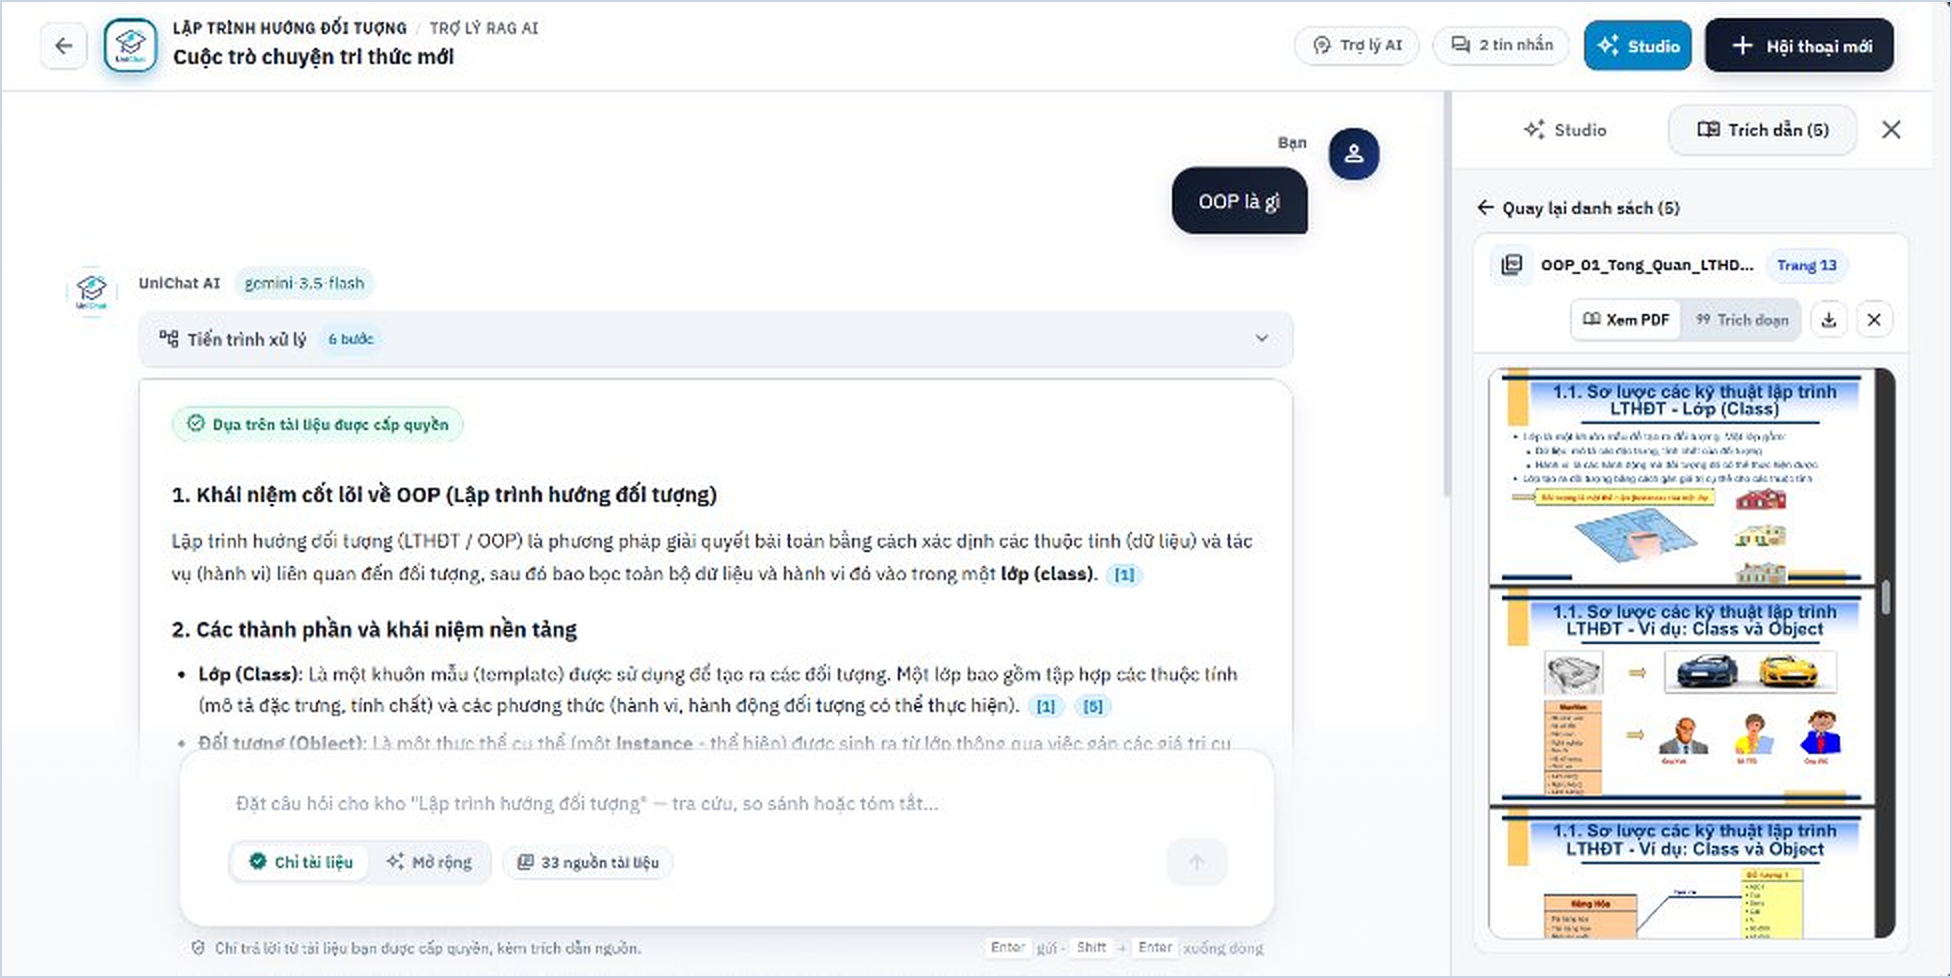
\includegraphics[width=0.92\textwidth]{chat_ui.png}
\caption{Giao diện hỏi đáp học liệu và ngăn đối chiếu trích dẫn (\textit{Knowledge Studio}) trên không gian môn học \textit{Lập trình hướng đối tượng} của UniChat: phản hồi từ mô hình \texttt{gemini-3.5-flash} hiển thị tiến trình xử lý 6 bước, huy hiệu \textit{``Dựa trên tài liệu được cấp quyền''}, chỉ số trích dẫn nội tuyến \texttt{[1]}, \texttt{[5]}, công tắc chế độ \textit{Chỉ tài liệu / Mở rộng} (33 nguồn tài liệu) và ngăn đối chiếu PDF mở trực tiếp trang tài liệu gốc (\texttt{OOP\_01\_Tong\_Quan\_LTHD...}, Trang 13) ở cột phải.}
\label{fig:chat_ui}
\end{figure*}

\textbf{3) Phân tích thống kê, độ lệch nhãn--kho tài liệu và kiểm định độ bám nguồn:}
Từ Bảng~\ref{tab:rag_benchmark} và đối chiếu dữ liệu thô, có sáu kết quả chính cần làm rõ:
\begin{enumerate}
    \item \textbf{Hiệu quả thực của đối chứng ghép cặp ($n=110$) và vai trò nhận diện ngoài phạm vi:} Khi loại trừ 10 câu lỗi JWT và chuẩn hóa 2 ca \texttt{DEFINITION} sót mẫu regex của \texttt{STRICT}, cả hai chế độ đạt độ chính xác nhận diện ý định bằng nhau ($97/110 = 88{,}2\%$, McNemar $p = 1{,}000$) và đều chặn đúng $12/12$ câu ngoài phạm vi hợp lệ (KTC 95\% Wilson: $75{,}8\%\text{--}100{,}0\%$). Khác biệt có ý nghĩa thống kê duy nhất đến từ chế độ sinh mở rộng có kiểm soát: $\text{Acc}_{\text{dec}}$ tăng từ $73{,}6\%$ lên $90{,}9\%$ (McNemar $b=1, c=20, p = 2{,}1\times 10^{-5} < 0{,}001$) và $\text{F1}_{\text{ref}}$ tăng từ $0{,}453$ lên $0{,}706$. Trên toàn bộ 120 câu ở chế độ \texttt{EXPANDED}, hệ thống chặn đúng $18/18$ câu hỏi ngoài phạm vi trên bộ thử nội bộ (KTC 95\%: $82{,}4\%\text{--}100{,}0\%$; gồm $12/12$ trên tập $\mathcal{D}_{\text{holdout}}$ với KTC $75{,}8\%\text{--}100{,}0\%$ và $6/6$ trên tập phát triển với KTC $61{,}0\%\text{--}100{,}0\%$), đồng thời từ chối $12/102$ ($11{,}8\%$) câu mang nhãn \texttt{ANSWER} ($\text{Prec}_{\text{ref}} = 18/30 = 60{,}0\%$, $\text{F1}_{\text{ref}} = 0{,}750$).
    \item \textbf{Báo cáo hai góc nhìn về độ lệch nhãn--kho tài liệu và phân biệt tập $\mathcal{D}_{\text{evid}}$ với $\mathcal{D}_{\text{holdout}}$:} Như đã chỉ ra ở Mục~\ref{subsec:golden_dataset}, mã câu \texttt{BM-QLDA-RSN-005} (\textit{Evidence Gate}) bị biên soạn nhầm vào không gian Quản lý dự án; nếu loại bỏ riêng ca gán nhãn sai này ($n=119$), độ chính xác quyết định của \texttt{EXPANDED} đạt $108/119 = 90{,}8\%$ (KTC 95\%: $84{,}2\%\text{--}94{,}8\%$). Đối chiếu giữa hai lượt chạy trên 98 câu trong phạm vi không lỗi JWT cho thấy \texttt{STRICT} (đã chuẩn hóa) trả lời trực tiếp từ slide tải lên trên \textbf{69 câu} và từ chối \textbf{29 câu} do slide nhập môn chưa chứa các chủ đề nâng cao đó. Để tránh nhầm lẫn với tập kiểm thử độc lập $\mathcal{D}_{\text{holdout}}$ ($n=81$, chỉ giao nhau trên 52 câu), ta đặt tên riêng \textbf{tập con đồng thuận chứng cứ $\mathcal{D}_{\text{evid}}$} ($n=81$, gồm $69$ câu trong phạm vi mà \texttt{STRICT} trả lời được cộng $12$ câu \texttt{OUT\_OF\_SCOPE} hợp lệ). Do $\mathcal{D}_{\text{evid}}$ được chọn theo điều kiện \texttt{STRICT} khớp quyết định, tỷ lệ $81/81$ của \texttt{STRICT} trên tập này chỉ là hệ quả của tiêu chí lọc, không phải kết quả đo độc lập (trên $\mathcal{D}_{\text{evid}}$, \texttt{STRICT} ghi nhận $\text{KHR}=58{,}5\%$); mục đích của $\mathcal{D}_{\text{evid}}$ là kiểm tra mức độ nhất quán của \texttt{EXPANDED} khi slide chắc chắn có bằng chứng: \texttt{EXPANDED} duy trì quyết định khớp trên \textbf{$80/81 = 98{,}8\%$ (KTC 95\%: $93{,}3\%\text{--}99{,}8\%$, $\text{KHR}=72{,}4\%$)}, chỉ từ chối quá mức duy nhất 1 ca là \texttt{BM-OOP-FACT-003} (từ khóa \texttt{static}). Ngược lại, trên 29 câu slide chưa có nội dung trực tiếp, \texttt{STRICT} từ chối cả 29/29 câu, trong khi \texttt{EXPANDED} từ chối 9/29 câu và vẫn trả lời \textbf{20/29 câu} bằng kiến thức nền mở rộng sau khi các đoạn liên quan chung của môn học vượt ngưỡng cổng bằng chứng -- mức tăng từ $73{,}6\%$ lên $90{,}9\%$ (và $90{,}0\%$ trên 120 câu) chủ yếu đến từ nhóm 20 câu này.
    \item \textbf{Đối chiếu tập phát triển (\texttt{DEVELOPMENT}) và tập kiểm thử độc lập $\mathcal{D}_{\text{holdout}}$:} Trên tập \texttt{DEVELOPMENT} ($n = 39$), \texttt{EXPANDED} đạt $\text{Acc}_{\text{int}} = 92{,}3\%$ ($36/39$, KTC 95\%: $79{,}7\%\text{--}97{,}3\%$) và $\text{Acc}_{\text{dec}} = 89{,}7\%$ ($35/39$, KTC 95\%: $76{,}4\%\text{--}95{,}9\%$). Trên tập kiểm thử độc lập $\mathcal{D}_{\text{holdout}}$ (\texttt{HOLDOUT}, $n = 81$), $\text{Acc}_{\text{int}} = 84{,}0\%$ ($68/81$, KTC 95\%: $74{,}5\%\text{--}90{,}4\%$) và $\text{Acc}_{\text{dec}} = 90{,}1\%$ ($73/81$, KTC 95\%: $81{,}7\%\text{--}94{,}9\%$). Do khoảng tin cậy 95\% của hai tập chồng lấp đáng kể ở cỡ mẫu hiện tại, hiệu số $8{,}3$ điểm phần trăm về nhận diện ý định chưa đủ cơ sở thống kê để kết luận quá khớp nghiêm trọng.
    \item \textbf{Kiểm định độ bám nguồn (faithfulness) thủ công trên mẫu phân tầng 30 câu trả lời:} Vì tỷ lệ hiện diện thẻ trích dẫn ($\text{CPR} = 96{,}1\%$) chưa đảm bảo tính trung thực ngữ nghĩa, chúng tôi chấm thủ công một mẫu phân tầng tất định gồm \textbf{30 câu đã trả lời} ở chế độ \texttt{EXPANDED} (10 câu/học phần, 2 câu/nhóm ý định trong phạm vi từ \texttt{benchmark-results.json}): có \textbf{$24/30$ câu ($80{,}0\%$, KTC 95\%: $62{,}7\%\text{--}90{,}5\%$)} bám trực tiếp nội dung slide được trích dẫn (được xác nhận trả lời trực tiếp ở cả \texttt{STRICT}); \textbf{$5/30$ câu ($16{,}7\%$)} (\texttt{BM-OOP-SUM-002}, \texttt{BM-OOP-RSN-002}, \texttt{BM-QLDA-FACT-001}, \texttt{BM-QLDA-CMP-003}, \texttt{BM-QLDA-RSN-001}) trả lời đúng chuyên môn nhờ kiến thức nền mở rộng dù \texttt{STRICT} báo thiếu trong slide -- đáng lưu ý là mô hình vẫn gắn thẻ trích dẫn vào các đoạn bài giảng liên quan gián tiếp, khẳng định bộ hậu kiểm cấu trúc hiện tại chưa thay thế được kiểm định suy luận ngữ nghĩa (NLI); và \textbf{$1/30$ câu ($3{,}3\%$)} (\texttt{BM-QLDA-FACT-003}) bị cắt cụt luồng ghi nhận ở dòng tiêu đề mục ($0$ trích dẫn).
    \item \textbf{Phân tích loại trừ ngoại tuyến (offline ablation) bộ điều phối ý định:} Do tệp kết quả Playwright DOM ngày 27/09/2026 không lưu mảng điểm cosine/từ vựng thô của từng ứng viên để tái lập toàn bộ nhánh truy xuất ngoại tuyến, chúng tôi thực hiện loại trừ ngoại tuyến trên mô-đun \texttt{intent\_detector.py} và \texttt{strategy\_selector.py} với đủ 120 câu hỏi (không tiêu tốn hạn ngạch LLM): (a) \textit{Đầy đủ bộ luật 6 ý định} đạt $\text{Acc}_{\text{int}} = 104/120$ ($86{,}7\%$), ngắt sớm $18/18$ câu \texttt{OUT\_OF\_SCOPE} ($0$ lượt gọi Chroma Cloud/LLM), ngân sách $\overline{\textit{Top-K}} = 6{,}45$ (trong phạm vi: $7{,}59$); (b) \textit{Loại bỏ luật \texttt{OUT\_OF\_SCOPE}} làm $\text{Acc}_{\text{int}}$ giảm còn $86/120$ ($71{,}7\%$), $0/18$ ca được ngắt sớm và phát sinh 18 truy vấn vector/LLM không cần thiết ($\overline{\textit{Top-K}} = 7{,}38$); (c) \textit{Cố định cấu hình kiểu Naive RAG (\texttt{FACT}, $\textit{Top-K}=5$)} chỉ khớp ngân sách $24/120$ ($20{,}0\%$) câu, không có ngắt sớm và cắt giảm $50\%\text{--}58\%$ ngân sách thu hồi của các câu \texttt{COMPARISON}, \texttt{SUMMARY}, \texttt{REASONING}. Kiểm tra bổ sung 78 vết truy xuất lưu trữ tại \texttt{retrieval\_traces.jsonl} ghi nhận 49 quyết định \texttt{ANSWER}, 20 \texttt{REFUSE} (10 ca không có tài liệu cấp quyền, 10 ca không đạt ngưỡng bằng chứng) và 9 \texttt{CLARIFY}.
    \item \textbf{Phân rã nguyên nhân độ trễ và tính minh bạch số lượt thử lại/dự phòng:} Phân tích nhật ký thực thi cho thấy các bước xử lý cục bộ chiếm thời gian nhỏ: phân loại ý định $< 15\text{~ms}$, truy xuất lai Chroma Cloud + RRF $0{,}45\text{--}1{,}20\text{~s}$, Evidence Gate $< 5\text{~ms}$. \textbf{Khoảng $90\%$} tổng thời gian chờ (trung bình $\approx 18\text{~s}$ trên $20{,}46\text{~s}$ ở \texttt{STRICT} [$n=110$] và $\approx 32\text{~s}$ trên $34{,}47\text{~s}$ ở \texttt{EXPANDED} [$N=120$]; P95 đạt $77{,}13\text{~s}$) nằm ở bước chờ dịch vụ Gemini sinh cấu trúc JSON dài và điều tiết giới hạn tần suất (rate-limit backoff) khi chạy liên tiếp 240 truy vấn; trên giao diện đơn lẻ, token tạm đầu tiên xuất hiện sau $1{,}35\text{--}2{,}45\text{~s}$ (Bảng~\ref{tab:functional_tests}). Cần lưu ý thẳng thắn rằng tệp kết quả DOM \texttt{benchmark-results.json} ngày 27/09/2026 không ghi bộ đếm riêng số lần \texttt{Citation Validator} phải thử lại hay chuyển khóa cho từng truy vấn; riêng nhật ký trace mạng Playwright xác nhận cơ chế chuyển đổi tự động từ \texttt{gemini-3.5-flash} sang \texttt{gemini-3.5-flash-lite} khi chạm giới hạn tần suất.
\end{enumerate}

\begin{figure*}[t]
\centering
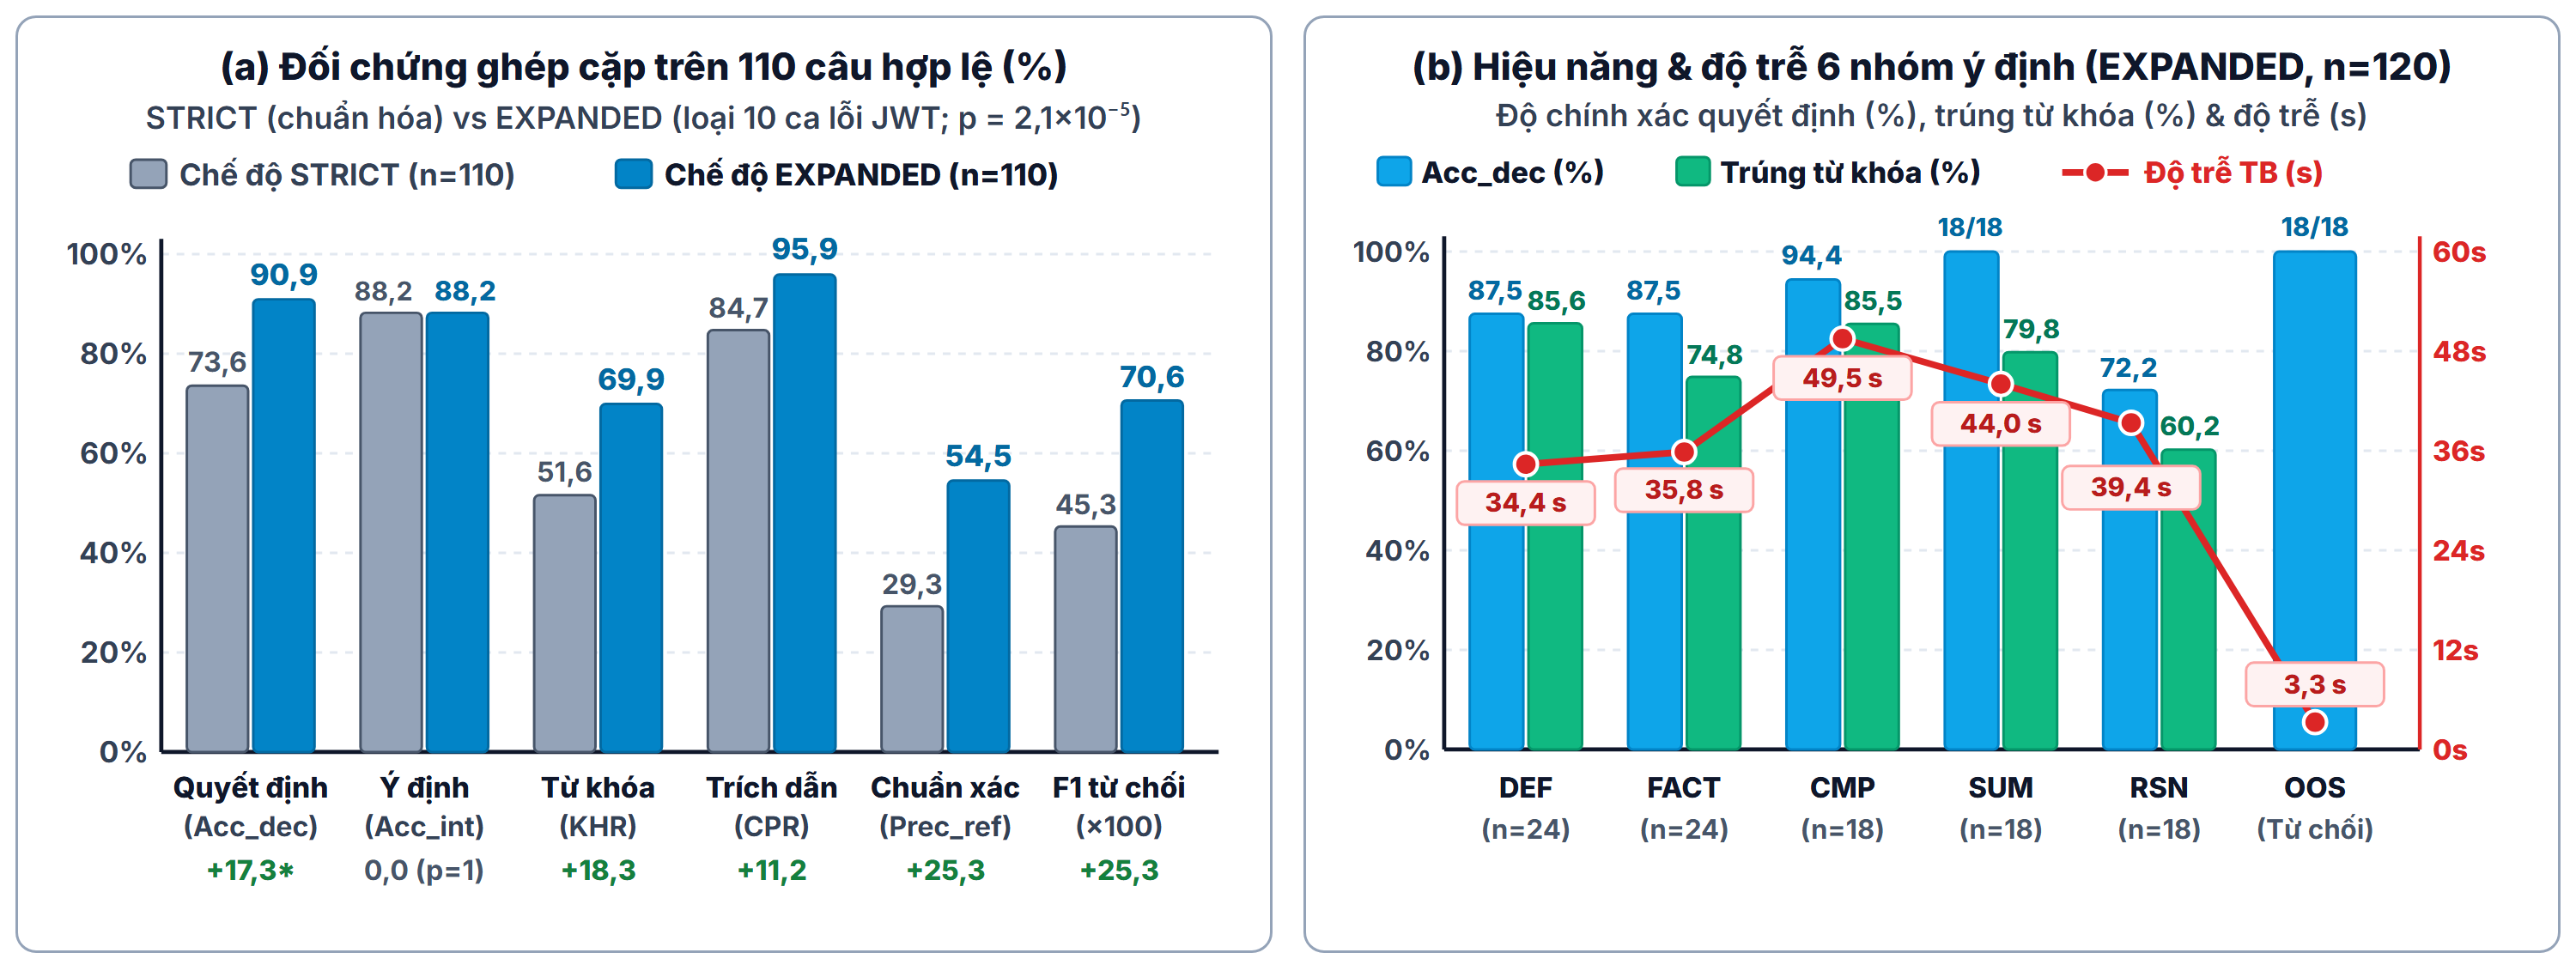
\includegraphics[width=0.92\textwidth]{rag_evaluation_charts.png}
\caption{Kết quả đánh giá thực nghiệm ngày 27/09/2026: (a) Đối chứng ghép cặp giữa chế độ \texttt{STRICT} (đã chuẩn hóa 2 ca \texttt{DEFINITION} sót regex) và \texttt{EXPANDED} trên 110 câu hợp lệ (loại 10 ca hết hạn JWT; McNemar $b=1, c=20, p=2{,}1\times 10^{-5}$ cho $\text{Acc}_{\text{dec}}$ và $p=1{,}000$ cho $\text{Acc}_{\text{int}}$); (b) Độ chính xác quyết định, tỷ lệ trúng từ khóa và độ trễ trung bình theo 6 nhóm ý định của \texttt{EXPANDED} trên toàn bộ 120 câu.}
\label{fig:rag_eval_charts}
\end{figure*}

\subsection{Phân tích theo nhóm ý định, ma trận nhầm lẫn và phân tích 12 ca lỗi}
\label{subsec:intent_and_error_analysis}
\textbf{1) Hiệu năng chi tiết theo từng nhóm ý định và chuẩn hóa nhóm \texttt{DEFINITION}:}
Bảng~\ref{tab:intent_breakdown} và Hình~\ref{fig:rag_eval_charts}b trình bày hiệu năng theo 6 nhóm ý định trên 110 câu ghép cặp hợp lệ của chế độ \texttt{STRICT} (đã chuẩn hóa) và toàn tập 120 câu của chế độ \texttt{EXPANDED}. Trên các nhóm \texttt{SUMMARY} ($18/18$) và \texttt{COMPARISON} ($17/18 = 94{,}4\%$), việc mở rộng ngân sách đoạn trích, tách khía cạnh truy vấn và bổ sung diễn giải có kiểm soát giúp tăng tỷ lệ trúng từ khóa từ $45{,}6\%$ và $61{,}1\%$ lên $79{,}8\%$ và $85{,}5\%$.

Đáng chú ý, trên nhóm \texttt{DEFINITION} ($n=24$), kết quả chấm tự động thô ban đầu ghi nhận \texttt{STRICT} đạt $23/24$ ($95{,}8\%$), có vẻ cao hơn \texttt{EXPANDED} ($21/24 = 87{,}5\%$). Tuy nhiên, kiểm tra trực tiếp văn bản câu trả lời trong \texttt{benchmark-results.json} chỉ ra đây là \textbf{điểm mù khớp chuỗi từ chối của trình chấm \texttt{chat-helper.ts}}: ở cả hai câu \texttt{BM-OOP-DEF-007} (\textit{Design Pattern}) và \texttt{BM-OOP-DEF-008} (\textit{SOLID}), chế độ \texttt{STRICT} thực tế cũng từ chối trả lời bằng cụm \textit{``không xuất hiện trong các tài liệu hiện có''} ($0$ trích dẫn, chưa có trong danh sách mẫu từ chối của trình chấm nên bị gán nhầm thành \texttt{ANSWER}), trong khi \texttt{EXPANDED} diễn đạt bằng cụm \textit{``nằm ngoài phạm vi tài liệu''} nên được nhận diện đúng là \texttt{REFUSE}. Vì vậy, toàn bộ bài báo (Tóm tắt, Bảng~\ref{tab:rag_benchmark}, Bảng~\ref{tab:intent_breakdown}, Hình~\ref{fig:rag_eval_charts}a và Kết luận) sử dụng thống nhất số liệu \texttt{STRICT} đã chuẩn hóa hai ca này: cả hai chế độ đều đạt $21/24$ ($87{,}5\%$) trên nhóm \texttt{DEFINITION}, tổng \texttt{STRICT} đạt $81/110$ ($73{,}6\%$), $\text{F1}_{\text{ref}} = 0{,}453$ và kiểm định McNemar hai phía cho $b=1, c=20, p = 2{,}1 \times 10^{-5}$. Đối với nhóm \texttt{OUT\_OF\_SCOPE}, dù hàm phân loại cú pháp ngắt sớm dưới $15\text{~ms}$, độ trễ toàn trình đo qua Playwright đạt trung bình $3{,}28\text{~s}$ (P50 $3{,}45\text{~s}$, P95 $4{,}23\text{~s}$) do bao gồm thao tác DOM, xác thực JWT, truy vấn quyền Supabase PostgreSQL 15, đóng luồng SSE và khoảng chờ ổn định DOM $500\text{~ms}$.

\begin{table*}[t]
\caption{Hiệu năng chi tiết theo 6 nhóm ý định: chế độ \texttt{STRICT} trên tập hợp lệ đã chuẩn hóa ($n=110$, loại 10 ca lỗi JWT) và chế độ \texttt{EXPANDED} trên toàn tập ($N=120$)}
\label{tab:intent_breakdown}
\centering
\scriptsize
\setlength{\tabcolsep}{3.0pt}
\begin{tabularx}{\textwidth}{|L{2.25cm}|C{0.95cm}|C{1.85cm}|C{1.75cm}|C{1.45cm}|C{1.45cm}|C{1.35cm}|C{1.35cm}|Y|}
\hline
\textbf{Nhóm ý định} & \textbf{Mẫu ($n_{110}/N$)} & \textbf{$\text{Acc}_{\text{dec}}$ (\texttt{STRICT}, $n_{110}$)} & \textbf{$\text{Acc}_{\text{dec}}$ (\texttt{EXPANDED}, $N$)} & \textbf{$\text{KHR}$ (\texttt{STRICT})} & \textbf{$\text{KHR}$ (\texttt{EXPANDED})} & \textbf{Trễ Avg (\texttt{STRICT})} & \textbf{Trễ Avg (\texttt{EXPANDED})} & \textbf{Phân vị trễ \texttt{EXPANDED} (P50 / P95)} \\
\hline
\texttt{DEFINITION} & 24 / 24 & 87,5\% (21/24)$^{\dagger}$ & 87,5\% (21/24) & 65,3\% & \textbf{85,6\%} & 25,85~s & 34,37~s & 29,72~s / 70,01~s \\
\texttt{FACT} & 24 / 24 & 66,7\% (16/24) & \textbf{87,5\%} (21/24) & 69,0\% & \textbf{74,8\%} & 26,18~s & 35,84~s & 34,10~s / 65,15~s \\
\texttt{COMPARISON} & 18 / 18 & 72,2\% (13/18) & \textbf{94,4\%} (17/18) & 61,1\% & \textbf{85,5\%} & 21,93~s & 49,50~s & 47,56~s / 79,55~s \\
\texttt{SUMMARY} & 18 / 18 & 66,7\% (12/18) & \textbf{18/18}$^{\ddagger}$ & 45,6\% & \textbf{79,8\%} & 20,09~s & 44,03~s & 41,59~s / 76,18~s \\
\texttt{REASONING} & 14 / 18 & 50,0\% (7/14) & \textbf{72,2\%} (13/18) & 38,2\% & \textbf{60,2\%} & 15,96~s & 39,35~s & 26,30~s / 97,19~s \\
\texttt{OUT\_OF\_SCOPE} & 12 / 18 & 12/12 & \textbf{18/18} & N/A & N/A & 1,81~s & 3,28~s & 3,45~s / 4,23~s \\
\hline
\textbf{Tổng / TB} & \textbf{110 / 120} & \textbf{73,6\% (81/110)} & \textbf{90,0\% (108/120)} & \textbf{51,6\%} & \textbf{65,9\%} & \textbf{20,46~s} & \textbf{34,47~s} & \textbf{32,11~s / 77,13~s} \\
\hline
\end{tabularx}
\vspace{2pt}
\begin{minipage}{\textwidth}
\scriptsize
$^{\dagger}$Số liệu \texttt{STRICT} đã chuẩn hóa 2 ca (\texttt{BM-OOP-DEF-007}, \texttt{DEF-008}) thực tế từ chối văn bản nhưng không khớp regex trình chấm (số thô trước chuẩn hóa: 23/24 = 95,8\%, tổng 83/110 = 75,5\%).\\
$^{\ddagger}$Gồm \texttt{BM-QLDA-SUM-006} mở đầu báo thiếu nội dung trong slide rồi bổ sung kiến thức mở rộng; trên 110 câu hợp lệ, \texttt{EXPANDED} đạt 11/14 (78,6\%) ở \texttt{REASONING} và 12/12 ở \texttt{OUT\_OF\_SCOPE}.
\end{minipage}
\end{table*}

\textbf{2) Ma trận nhầm lẫn $6 \times 6$ của bộ nhận diện ý định:}
Bảng~\ref{tab:confusion_matrix} trình bày ma trận nhầm lẫn $6 \times 6$ trên toàn bộ 120 câu hỏi (tổng số câu phân loại đúng đạt $23 + 19 + 15 + 18 + 11 + 18 = 104/120 = 86{,}7\%$, KTC 95\% Wilson: $79{,}4\%\text{--}91{,}6\%$). Ma trận cho thấy hai hiện tượng chính: (i) không có câu hỏi học thuật nào bị nhận nhầm thành \texttt{OUT\_OF\_SCOPE} và cả $18/18$ câu ngoài phạm vi được tách biệt chính xác; (ii) phần lớn các ca nhầm lẫn ($11/16$ ca sai, gồm $7$ ca của \texttt{REASONING}, $3$ ca của \texttt{COMPARISON} và $1$ ca của \texttt{DEFINITION}) rơi vào cột mặc định \texttt{FACT}. Nguyên nhân là các câu hỏi này mở đầu bằng động từ phân tích (\textit{``Phân tích ưu và nhược điểm...''}, \textit{``Giải thích vai trò...''}, \textit{``Khi nào nên dùng...''}) nhưng không chứa từ khóa nguyên nhân tường minh trong bộ luật YAML v1.0, nên rơi xuống nhánh mặc định \texttt{FACT\_DEFAULT}.

\begin{table}[t]
\caption{Ma trận nhầm lẫn $6 \times 6$ của bộ phân loại ý định trên 120 câu hỏi (hàng: nhãn chuẩn, cột: nhãn dự đoán; độ chính xác 104/120 = 86,7\%)}
\label{tab:confusion_matrix}
\centering
\scriptsize
\setlength{\tabcolsep}{2.0pt}
\begin{tabularx}{\columnwidth}{|L{2.42cm}|Z|Z|Z|Z|Z|Z|C{0.82cm}|}
\hline
\textbf{Chuẩn $\backslash$ Dự đoán} & \textbf{DEF} & \textbf{FACT} & \textbf{CMP} & \textbf{SUM} & \textbf{RSN} & \textbf{OOS} & \textbf{Đúng} \\
\hline
\texttt{DEFINITION} (24) & \textbf{23} & 1 & 0 & 0 & 0 & 0 & 23/24 \\
\texttt{FACT} (24) & 3 & \textbf{19} & 1 & 0 & 1 & 0 & 19/24 \\
\texttt{COMPARISON} (18) & 0 & 3 & \textbf{15} & 0 & 0 & 0 & 15/18 \\
\texttt{SUMMARY} (18) & 0 & 0 & 0 & \textbf{18} & 0 & 0 & 18/18 \\
\texttt{REASONING} (18) & 0 & 7 & 0 & 0 & \textbf{11} & 0 & 11/18 \\
\texttt{OUT\_OF\_SCOPE} (18) & 0 & 0 & 0 & 0 & 0 & \textbf{18} & 18/18 \\
\hline
\end{tabularx}
\end{table}

\textbf{3) Phân tích nguyên nhân 12 câu hỏi có quyết định \texttt{REFUSE} trên nhãn gốc \texttt{ANSWER}:}
Đối chiếu trực tiếp từng bản ghi trong \texttt{benchmark-results.json} cho phép phân tách 12 ca này thành ba nhóm nguyên nhân thực tế:
\begin{enumerate}
    \item \textit{Lỗi gán nhãn đặt nhầm câu hỏi ngoài môn học (1/12 ca):} Mã ca \texttt{BM-QLDA-RSN-005} (\textit{``Giải thích vai trò của Evidence Gate trong đánh giá chất lượng retrieval?''}) hỏi về thành phần của chính UniChat nhưng bị đặt vào không gian môn Quản lý dự án và gán nhãn \texttt{ANSWER}; việc hệ thống từ chối thực chất là hành vi đúng với kho tài liệu.
    \item \textit{Thiếu nội dung tương ứng trong slide bài giảng tải lên, kèm thu hẹp ngân sách do nhận diện nhầm ý định (10/12 ca):} Gồm 4 ca bị nhầm từ \texttt{REASONING} sang \texttt{FACT} (\texttt{BM-OOP-RSN-003} Singleton Pattern, \texttt{BM-MDB-RSN-003} embedding vs referencing, \texttt{BM-MDB-RSN-004} MongoDB vs RDBMS, \texttt{BM-QLDA-RSN-003} ưu/nhược điểm Agile) và 6 ca nhận diện đúng ý định (\texttt{BM-OOP-DEF-007} Design Pattern, \texttt{BM-OOP-DEF-008} SOLID, \texttt{BM-OOP-FACT-004} \texttt{finalize()}, \texttt{BM-QLDA-DEF-006} quản lý rủi ro, \texttt{BM-QLDA-FACT-002} số lĩnh vực PMBOK, \texttt{BM-QLDA-CMP-002} Scrum vs Kanban). Ở toàn bộ các ca không lỗi phiên trong nhóm này, cả hai chế độ \texttt{STRICT} và \texttt{EXPANDED} đều báo rõ rằng các slide bài giảng nhập môn tải lên không đề cập trực tiếp các chủ đề trên. (Ngoài ra, \texttt{BM-QLDA-SUM-006} về quản lý truyền thông dự án cũng thiếu trong slide nhưng được \texttt{EXPANDED} bổ sung kiến thức mở rộng sau câu thông báo thiếu nguồn).
    \item \textit{Từ chối quá mức thực sự trên câu hỏi có bằng chứng trong slide (1/12 ca):} Chỉ duy nhất \texttt{BM-OOP-FACT-003} (\textit{``Từ khóa \texttt{static} trong Java có tác dụng gì?''}) xuất hiện trong đoạn mã ví dụ \texttt{static void main} của bài giảng (được xác nhận qua việc chế độ \texttt{STRICT} đã trích xuất và trả lời đúng), nhưng bị chế độ \texttt{EXPANDED} từ chối.
\end{enumerate}

\subsection{Bàn luận và hạn chế của nghiên cứu}
\label{subsec:discussion_limitations}
Bên cạnh những kết quả đạt được trong việc tích hợp trợ lý hỏi đáp có trích dẫn vào môi trường thảo luận học tập, nghiên cứu hiện tại còn tồn tại sáu hạn chế cần được nhìn nhận thẳng thắn:
\begin{enumerate}
    \item \textbf{Chưa có đối chứng trực tiếp với Naive RAG độc lập và ảnh hưởng của sự cố hết hạn JWT trong lượt \texttt{STRICT}:} Lượt chạy \texttt{STRICT} ngày 27/09/2026 là chế độ chỉ tài liệu của chính UniChat (không phải Naive RAG \textit{Top-K} cố định) và gặp lỗi hết hạn JWT ở 10 câu cuối môn Quản lý dự án. Dù bài báo đã khắc phục phân tích bằng đối chứng ghép cặp McNemar trên 110 câu hợp lệ và thực hiện phân tích loại trừ ngoại tuyến bộ điều phối ý định, nghiên cứu chưa chạy thêm lượt thực nghiệm đầu-cuối độc lập với cấu hình Naive RAG thuần trên cùng ảnh chụp mô hình (do mã \texttt{gemini-3.5-flash} đã được chuyển hướng sang \texttt{gemini-3.6-flash}).
    \item \textbf{Độ lệch nhãn--kho tài liệu và tính dễ nhận diện của 18 câu ngoài phạm vi:} Bộ 120 câu do chính hai sinh viên đồng tác giả biên soạn theo đề cương nên phát sinh ca gán nhãn nhầm \texttt{BM-QLDA-RSN-005} và nhiều câu hỏi nâng cao vượt quá phạm vi slide nhập môn thực tế tải lên. Do các tệp slide gốc lưu tách biệt trên kho đám mây và chưa gắn siêu dữ liệu số trang vào tệp JSON kiểm thử, bài báo sử dụng đối chiếu qua chế độ \texttt{STRICT} kết hợp chấm tay 30 câu để tách tập con đồng thuận chứng cứ $\mathcal{D}_{\text{evid}}$ ($n=81$, tách biệt với $\mathcal{D}_{\text{holdout}}$; tỷ lệ khớp của \texttt{STRICT} trên $\mathcal{D}_{\text{evid}}$ là hệ quả của tiêu chí lọc, không phải kết quả đo độc lập) thay vì lập bảng ánh xạ trang thủ công cho đủ 102 câu. Đồng thời, 18 câu \texttt{OUT\_OF\_SCOPE} chủ yếu thuộc chủ đề đời sống dễ bắt bằng từ khóa; cần bổ sung các câu hỏi ngoài phạm vi khó hơn (cùng ngành CNTT nhưng ngoài giáo trình hoặc có prompt injection) ở phiên bản kiểm thử tiếp theo để đánh giá chặt chẽ năng lực chặn của cổng bằng chứng.
    \item \textbf{Hạn chế của bộ phân loại dựa trên luật và việc ghép chung hai thang điểm tại Evidence Gate:} Bộ phân loại cú pháp mới đạt $11/18$ ($61{,}1\%$) trên nhóm \texttt{REASONING}. Về cổng bằng chứng, bất đẳng thức~(\ref{eq:floor_bound}) cho thấy ngưỡng \textit{Gate} bị che khuất bởi \textit{Floor} trên nhánh vector thuần túy, trong khi việc đưa trực tiếp hai thang đo khác bản chất ($s^{\text{dense}}$ cosine và $s^{\text{lex}}$ chồng lấp từ vựng) vào cùng một công thức tuyến tính và cùng ngưỡng \textit{Gate} dễ gây lệch điểm như minh họa ở ca \texttt{BM-OOP-FACT-004}.
    \item \textbf{Khoảng cách giữa hậu kiểm cấu trúc và độ trung thực ngữ nghĩa ở chế độ Mở rộng:} Kiểm định thủ công trên 30 câu trả lời cho thấy $24/30$ ($80{,}0\%$) câu bám sát tài liệu, nhưng $5/30$ ($16{,}7\%$) câu ở chế độ \texttt{EXPANDED} dùng kiến thức nền khi slide thiếu nội dung mà vẫn đính thẻ trích dẫn liên quan gián tiếp, và $1/30$ câu bị cắt cụt hiển thị. Ngoài ra, tệp kết quả DOM chưa ghi bộ đếm số lượt thử lại \texttt{Citation Validator} cho đủ 240 truy vấn. Việc đo lường tự động độ trung thực ngữ nghĩa (\textit{faithfulness}) theo khung RAGAS \cite{es2024ragas} và lưu vết đầy đủ số lượt retry/fallback là bước bắt buộc tiếp theo.
    \item \textbf{Phạm vi kiểm thử tải còn hẹp:} Bài kiểm thử tải HTTP chỉ chạy trên endpoint \texttt{/api/auth/login} (chủ yếu đo chi phí băm BCrypt và ký JWT) chứ chưa đo tải đồng thời cho các endpoint đọc diễn đàn hay luồng suy luận RAG.
    \item \textbf{Độ trễ toàn trình còn cao và chưa khảo sát người dùng cuối:} Độ trễ hoàn tất trung bình $34{,}47\text{~s}$ (P95 $77{,}13\text{~s}$) khi sinh JSON dài là rào cản với lớp học đông sinh viên; hệ thống cũng chưa triển khai khảo sát thực địa theo thang đo khả dụng SUS với sinh viên trong học kỳ thực tế.
\end{enumerate}

\section{Kết luận và hướng phát triển}
\label{sec:conclusion}
Bài báo đã trình bày quá trình thiết kế, triển khai và đánh giá thực nghiệm nền tảng thảo luận học tập \textbf{UniChat} tích hợp trợ lý AI trả lời có trích dẫn từ tài liệu môn học. Hệ thống kết hợp diễn đàn phân nhánh, bày tỏ cảm xúc, nhắn tin trực tiếp qua WebSocket và cơ chế triệu hồi \texttt{@UniChat} dưới sự kiểm soát của ma trận phân quyền RBAC trên kiến trúc 4 tầng. Về mặt xử lý truy vấn học liệu, hệ thống áp dụng và điều chỉnh bộ phân loại 6 nhóm ý định tiếng Việt kết hợp truy xuất lai (vector \texttt{intfloat/multilingual-e5-base} trên Chroma Cloud và khớp từ vựng hợp nhất qua RRF), cổng kiểm tra bằng chứng và bộ hậu kiểm trích dẫn có cơ chế thu hồi luồng tạm (\texttt{SSE reset}).

Đánh giá tự động ngày 27/09/2026 trên bộ 120 câu hỏi tiếng Việt thuộc 3 học phần cho thấy chế độ mở rộng có kiểm soát (\texttt{EXPANDED}) đạt độ chính xác quyết định $90{,}0\%$ ($108/120$, KTC 95\% Wilson: $83{,}3\%\text{--}94{,}2\%$; tập kiểm thử độc lập $\mathcal{D}_{\text{holdout}}$ 81 câu đạt $90{,}1\%$, KTC $81{,}7\%\text{--}94{,}9\%$), nhận diện ý định $86{,}7\%$ ($104/120$, KTC $79{,}4\%\text{--}91{,}6\%$), chặn đúng $18/18$ câu hỏi ngoài phạm vi nội bộ (KTC 95\%: $82{,}4\%\text{--}100{,}0\%$; $\text{Prec}_{\text{ref}} = 60{,}0\%$, $\text{F1}_{\text{ref}} = 0{,}750$) và hiện diện trích dẫn $96{,}1\%$ ($98/102$). Trên 110 câu ghép cặp hợp lệ, \texttt{EXPANDED} đạt độ chính xác quyết định cao hơn \texttt{STRICT} đã chuẩn hóa ($90{,}9\%$ so với $73{,}6\%$, McNemar $b=1, c=20, p = 2{,}1\times 10^{-5}$; $\text{F1}_{\text{ref}}$ $0{,}706$ so với $0{,}453$), song mức tăng này chủ yếu đến từ 20/29 câu thiếu nội dung trực tiếp trong slide mà \texttt{EXPANDED} trả lời bằng kiến thức nền; trên tập con đồng thuận chứng cứ $\mathcal{D}_{\text{evid}}$ ($n=81$, khác với $\mathcal{D}_{\text{holdout}}$), \texttt{EXPANDED} duy trì độ nhất quán $80/81$ ($98{,}8\%$). Kiểm định thủ công mẫu phân tầng 30 câu trả lời xác nhận $24/30$ ($80{,}0\%$) câu bám trực tiếp tài liệu nguồn. Kiểm thử tải xác thực trên API đăng nhập đạt $324{,}45\text{~req/s}$ ở 200 kết nối đồng thời không lỗi.

Trong giai đoạn tiếp theo, nhóm nghiên cứu tập trung vào bốn hướng cải tiến:
\begin{itemize}
    \item Chuẩn hóa lại bộ dữ liệu đánh giá gắn tọa độ trang/slide chứng cứ cho từng câu hỏi, bổ sung nhóm câu ngoài phạm vi khó (cùng ngành và prompt injection), và kết hợp mô hình ngôn ngữ gọn nhẹ với luật cú pháp để khắc phục nhầm lẫn ở nhóm \texttt{REASONING} cùng chuẩn hóa riêng hai thang điểm vector/từ vựng tại Evidence Gate.
    \item Chạy thực nghiệm đối chứng độc lập với Naive RAG thuần và nghiên cứu loại trừ toàn trình có ghi nhận đầy đủ bộ đếm retry/fallback, kết hợp đánh giá tự động độ trung thực ngữ nghĩa (\textit{faithfulness}) theo khung RAGAS \cite{es2024ragas}.
    \item Tối ưu độ trễ sinh văn bản bằng bộ nhớ đệm ngữ nghĩa (semantic caching), rút gọn lược đồ JSON đầu ra và mở rộng kiểm thử tải sang các endpoint đọc diễn đàn cùng luồng RAG.
    \item Tích hợp nhận dạng ký tự quang học (OCR) cho tài liệu bản quét và tổ chức triển khai thử nghiệm thực địa với sinh viên lớp học phần theo thang đo SUS.
\end{itemize}

\section*{Tính sẵn sàng của dữ liệu và khai báo sử dụng AI}
Mã nguồn của nền tảng UniChat, bộ dữ liệu 120 câu hỏi đánh giá (\texttt{automation-tests/data/golden-dataset.json}), kịch bản kiểm thử Playwright E2E và tệp kết quả thực nghiệm thô (\texttt{benchmark-results.json}) được lưu trữ tại kho mã nguồn dự án \url{https://github.com/Hiep0718/unichat}. Trong quá trình chuẩn bị và hoàn thiện bản thảo, nhóm tác giả có sử dụng công cụ trí tuệ nhân tạo tạo sinh để hỗ trợ rà soát diễn đạt tiếng Việt/tiếng Anh, định dạng mã nguồn \LaTeX{} và kiểm tra đối chiếu số liệu từ nhật ký thực nghiệm; toàn bộ mã nguồn hệ thống, số liệu đo kiểm, công thức toán học và danh mục 23 tài liệu tham khảo ở bản sửa đổi cuối cùng đã được nhóm tác giả rà soát trực tiếp đối chiếu với nguồn gốc (ACL Anthology, IEEE Xplore, arXiv và tài liệu chính thức của các nền tảng) và chịu hoàn toàn trách nhiệm về tính chính xác khoa học.

\section*{Lời cảm ơn}
Nhóm tác giả xin trân trọng cảm ơn Ban Chủ nhiệm và các giảng viên Khoa Công nghệ Thông tin, Trường Đại học Công nghiệp TP. Hồ Chí Minh (IUH) đã tạo điều kiện học thuật thuận lợi, cung cấp học liệu tham khảo và những góp ý chuyên môn sâu sắc giúp nhóm hoàn thiện nghiên cứu này.

\balance
\begin{thebibliography}{00}
\setlength{\itemsep}{0.5pt}
\setlength{\parskip}{0pt}
\bibitem{lewis2020rag} P. Lewis, E. Perez, A. Piktus, F. Petroni, V. Karpukhin, N. Goyal, \textit{et al.}, ``Retrieval-augmented generation for knowledge-intensive NLP tasks,'' in \textit{Advances in Neural Information Processing Systems (NeurIPS)}, vol. 33, pp. 9459--9474, 2020.
\bibitem{gao2023rag} Y. Gao, Y. Xiong, X. Gao, K. Jia, J. Pan, Y. Bi, \textit{et al.}, ``Retrieval-augmented generation for large language models: A survey,'' \textit{arXiv preprint arXiv:2312.10997}, Dec. 2023.
\bibitem{huang2025survey} L. Huang, W. Yu, W. Ma, W. Zhong, Z. Feng, H. Wang, \textit{et al.}, ``A survey on hallucination in large language models: Principles, taxonomy, challenges, and open questions,'' \textit{ACM Trans. Inf. Syst.}, vol. 43, no. 2, Art. no. 42, pp. 1--55, Mar. 2025, doi: 10.1145/3703155.
\bibitem{jeong2024adaptiverag} S. Jeong, J. Baek, S. Cho, S. J. Hwang, and J. C. Park, ``Adaptive-RAG: Learning to adapt retrieval-augmented large language models through question complexity,'' in \textit{Proc. Conf. North Amer. Chapter Assoc. Comput. Linguist.: Hum. Lang. Technol. (NAACL-HLT)}, Jun. 2024, pp. 7036--7050, doi: 10.18653/v1/2024.naacl-long.389.
\bibitem{asai2024selfrag} A. Asai, Z. Wu, Y. Wang, A. Sil, and H. Hajishirzi, ``Self-RAG: Learning to retrieve, generate, and critique through self-reflection,'' in \textit{Proc. Int. Conf. Learn. Represent. (ICLR)}, May 2024.
\bibitem{yan2024crag} S.-Q. Yan, J.-C. Gu, Y. Zhu, and Z.-H. Ling, ``Corrective retrieval augmented generation,'' \textit{arXiv preprint arXiv:2401.15884}, Jan. 2024.
\bibitem{moodle_ai} Moodle Docs, ``AI subsystem,'' Moodle 4.5+ Documentation, 2024. [Online]. Available: \url{https://docs.moodle.org/en/AI_subsystem}. Accessed: Nov. 21, 2026.
\bibitem{piazza_ai} UCLA Digital \& Technology Solutions, ``Piazza Enhancement: AI Summaries,'' Sep. 2026. [Online]. Available: \url{https://dts.ucla.edu/news/piazza-enhancement-ai-summaries}. Accessed: Nov. 21, 2026.
\bibitem{notebooklm_share} Google Support, ``Share a notebook in NotebookLM,'' NotebookLM Help, 2026. [Online]. Available: \url{https://support.google.com/notebooklm/answer/16206563}. Accessed: Nov. 21, 2026.
\bibitem{nguyen2024virag} Q. D. Nguyen, H. S. Le, D. N. Nguyen, D. N. M. Nguyen, T. H. Le, and V. S. Dinh, ``Towards comprehensive Vietnamese retrieval-augmented generation and large language models,'' \textit{arXiv preprint arXiv:2403.01616}, Mar. 2024.
\bibitem{cormack2009rrf} G. V. Cormack, C. L. Clarke, and S. Buettcher, ``Reciprocal rank fusion outperforms condorcet and individual rank learning methods,'' in \textit{Proc. 32nd Int. ACM SIGIR Conf. Res. Develop. Inf. Retr.}, Jul. 2009, pp. 758--759, doi: 10.1145/1571941.1572114.
\bibitem{wang2024multilinguale5} L. Wang, N. Yang, X. Huang, L. Yang, R. Majumder, and F. Wei, ``Multilingual E5 text embeddings: A technical report,'' \textit{arXiv preprint arXiv:2402.05672}, Feb. 2024.
\bibitem{react_docs} Meta Platforms, Inc., ``React Documentation: Describing the UI,'' \textit{React Official}, 2024. [Online]. Available: \url{https://react.dev/}. Accessed: Nov. 9, 2026.
\bibitem{spring_boot_docs} Broadcom Inc., ``Spring Boot Reference Documentation,'' \textit{VMware Tanzu}, 2024. [Online]. Available: \url{https://docs.spring.io/spring-boot/index.html}. Accessed: Nov. 9, 2026.
\bibitem{jwt2015rfc} M. Jones, J. Bradley, and N. Sakimura, ``JSON Web Token (JWT),'' \textit{IETF RFC 7519}, May 2015, doi: 10.17487/RFC7519.
\bibitem{rfc9457} M. Nottingham, E. Wilde, and S. Dalal, ``Problem details for HTTP APIs,'' \textit{IETF RFC 9457} (obsoletes RFC 7807, Mar. 2016), Jul. 2023, doi: 10.17487/RFC9457.
\bibitem{fastapi_docs} S. Ramírez, ``FastAPI Framework, high performance, easy to learn, fast to code, ready for production,'' 2024. [Online]. Available: \url{https://fastapi.tiangolo.com/}. Accessed: Nov. 9, 2026.
\bibitem{kleppmann2017designing} M. Kleppmann, \textit{Designing Data-Intensive Applications: The Big Ideas Behind Reliable, Scalable, and Maintainable Systems}. Sebastopol, CA, USA: O'Reilly Media, 2017.
\bibitem{chroma_docs} Chroma Core Team, ``Chroma: The AI-native open-source embedding database,'' 2024. [Online]. Available: \url{https://docs.trychroma.com/}. Accessed: Nov. 9, 2026.
\bibitem{karpukhin2020dpr} V. Karpukhin, B. Oguz, S. Min, P. Lewis, L. Wu, \textit{et al.}, ``Dense passage retrieval for open-domain question answering,'' in \textit{Proc. Conf. Empirical Methods Natural Lang. Process. (EMNLP)}, Nov. 2020, pp. 6769--6781, doi: 10.18653/v1/2020.emnlp-main.550.
\bibitem{malkov2020hnsw} Yu. A. Malkov and D. A. Yashunin, ``Efficient and robust approximate nearest neighbor search using Hierarchical Navigable Small World graphs,'' \textit{IEEE Trans. Pattern Anal. Mach. Intell.}, vol. 42, no. 4, pp. 824--836, Apr. 2020, doi: 10.1109/TPAMI.2018.2889473.
\bibitem{cohen1960kappa} J. Cohen, ``A coefficient of agreement for nominal scales,'' \textit{Educ. Psychol. Meas.}, vol. 20, no. 1, pp. 37--46, Apr. 1960, doi: 10.1177/001316446002000104.
\bibitem{es2024ragas} S. Es, J. James, L. Espinosa-Anke, and S. Schockaert, ``RAGAS: Automated evaluation of retrieval augmented generation,'' in \textit{Proc. 18th Conf. Eur. Chapter Assoc. Comput. Linguist. (EACL): Syst. Demonstrations}, Mar. 2024, pp. 150--158, doi: 10.18653/v1/2024.eacl-demo.16.
\end{thebibliography}

\end{document}
